\chapter{Interferometric methods for tokamak-plasma fluctuations}
Interferometric methods exploit the interaction of
electromagnetic waves with a plasma
to ascertain properties of the plasma's density.
Because surveying every flavor of interferometric method
exceeds the scope of this work,
only the interferometric methods
of direct relevance to this work ---
external reference-beam interferometry and phase contrast imaging (PCI) ---
are discussed in detail.
Further, the emphasis will be on the diagnosis of
the plasma's density fluctuations rather than its equilibrium.

Below, Section~\ref{sec:InterferometricMethods:EM_waves_in_plasma}
examines the propagation of electromagnetic waves through a ``cold'' plasma
and derives an expression for the plasma-induced phase delay.
Section~\ref{sec:InterferometricMethods:Gaussian_beam_diffraction} reveals that
plasma-density fluctuations weakly upscatter an downscatter
an incident Gaussian probe beam, while
Section~\ref{sec:InterferometricMethods:imaging} describes
how an imaging system manipulates these scattered beams.
Section~\ref{sec:InterferometricMethods:interferometry} shows that
interfering the imaged probe radiation with an external reference beam
is an effective technique for diagnosing plasma-density fluctuations and
discusses the relative merits of homodyne versus heterodyne detection.
Section~\ref{sec:InterferometricMethods:pci} details the principles of
phase contrast imaging (PCI),
which does away with an external reference beam and
instead applies careful spatial filtering
of the scattered and unscattered beams
to produce its diagnosing interference signal;
further, this section and Appendix~\ref{app:PCIResponseIdentities}
derive the PCI transfer function across the full beam profile, which
is needed to correctly account for PCI's low-$k$ behavior and is,
to the author's knowledge, the first such complete derivation.
Section~\ref{sec:InterferometricMethods:selection}
concludes the chapter by synthesizing the preceding results and
discussing the strengths and limitations of each interferometric technique.


\section{Electromagnetic waves in a plasma}
\label{sec:InterferometricMethods:EM_waves_in_plasma}
A great deal can be learned about a plasma
by probing it with electromagnetic waves.
Sections~\ref{sec:InterferometricMethods:EM_waves_in_plasma:derivation_of_wave_equation}---
\ref{sec:InterferometricMethods:EM_waves_in_plasma:cold_plasma_dispersion_relation}
derive the index of refraction $N$ for a cold, homogeneous plasma.
Section~\ref{sec:InterferometricMethods:EM_waves_in_plasma:propagation_in_inhomogeneous_medium}
extends these results to inhomogeneous plasmas via the WKB approximation and
assesses the validity of this approach for
a CO$_2$ probe beam in a typical tokamak plasma, and
Section~\ref{sec:InterferometricMethods:EM_waves_in_plasma:plasma_induced_phase_delay}
computes the resulting plasma-induced phase delay.


\subsection{Derivation of the wave equation}
\label{sec:InterferometricMethods:EM_waves_in_plasma:derivation_of_wave_equation}
An electromagnetic wave's electric and magnetic fields
are related via Faraday's law
\begin{equation}
  \nabla \cross \vect{E} = - \frac{\partial \vect{B}}{\partial t}.
  \label{eq:InterferometricMethods:Faradays_law}
\end{equation}
Taking the curl of Faraday's law
(\ref{eq:InterferometricMethods:Faradays_law}) and
using Ampere's law to eliminate $\vect{B}$ yields
the electric field's wave equation
\begin{equation}
  \nabla^2 \vect{E}
  -
  \frac{1}{c^2} \frac{\partial^2 \vect{E}}{\partial t^2}
  =
  \nabla(\nabla \cdot \vect{E})
  +
  \mu_0 \frac{\partial \vect{J}}{\partial t},
\end{equation}
where $\mu_0$ is the permeability of free space.
The current density $\vect{J}$ is related to the electric field via
\begin{equation}
  \vect{J} = \vect{\sigma} \cdot \vect{E},
  \label{eq:InterferometricMethods:current_density_sigma_E}
\end{equation}
where $\vect{\sigma}$ is the conductivity of the surrounding medium.
Typically, the electromagnetic wave's oscillations occur on timescales
that are orders-of-magnitude faster than any changes to the medium, and
the wave equation becomes
\begin{equation}
  \nabla^2 \vect{E}
  -
  \frac{1}{c^2} \frac{\partial^2 \vect{E}}{\partial t^2}
  =
  \nabla(\nabla \cdot \vect{E})
  +
  \mu_0 \vect{\sigma} \cdot \frac{\partial \vect{E}}{\partial t}.
  \label{eq:InterferometricMethods:wave_equation_pde}
\end{equation}


\subsection{Wave equation in a homogeneous medium}
Assume that the medium is homogeneous in space and time such that
the field can be Fourier analyzed~\cite[Sec.~3-2]{stix}
\begin{equation}
  \vect{E}(\vect{r}, t)
  =
  \frac{1}{(2 \pi)^4}
  \int
  \vect{E}(\vect{k}', \omega')
  e^{i(\vect{k}' \cdot \vect{r} - \omega' t)}
  d\vect{k'} \, d\omega'.
\end{equation}
Then, the electric field's wave equation
(\ref{eq:InterferometricMethods:wave_equation_pde}) reduces
to an algebraic equation for each Fourier component.
In particular, for Fourier mode
$\vect{E}_0 e^{i(\vect{k} \cdot \vect{r} - \omega t)}$,
the derivative operators become
$\nabla \rightarrow i \vect{k}$ and
$\partial / \partial t \rightarrow -i \omega$, and
the wave equation reduces to an eigenvalue equation
\begin{equation}
  \left[%
    \vect{N}\vect{N}
    -
    N^2\vect{I}
    +
    \left(%
      \vect{I}
      +
      \frac{i \vect{\sigma}}{\varepsilon_0 \omega}
    \right)
  \right]
  \cdot
  \vect{E}_0
  =
  0,
  \label{eq:InterferometricMethods:wave_equation_eigenvalue}
\end{equation}
where
\begin{equation}
  \vect{N} \equiv \frac{c \vect{k}}{\omega}
  \label{eq:InterferometricMethods:refraction_index}
\end{equation}
is the index of refraction seen by the given Fourier mode,
$\varepsilon_0$ is the permittivity of free space, and
$\vect{I}$ is the identity matrix.
To proceed further, a model is needed
for the medium's conductivity $\vect{\sigma}$.


\subsection{The cold-plasma index of refraction}
\label{sec:InterferometricMethods:EM_waves_in_plasma:cold_plasma_dispersion_relation}
Although plasmas in contemporary fusion devices
routinely approach temperatures $\lesssim 100$ million degrees Celsius
($\sim10\times$ the temperature of the core of the sun!),
the thermal velocities of the constituent particles are
still far below the speed of light.
The lightest, and consequently the fastest,
of such a plasma's constituent particles are its electrons,
which have thermal velocities $\lesssim 0.1 c$.
In contrast, as will be shown shortly,
the electromagnetic waves used to make interferometric measurements
in such plasmas have phase velocities very close to the speed of light.
Thus, in the context of the wave-plasma interaction,
the unperturbed plasma can be modeled as a collection
of motionless (i.e.\ zero-temperature or ``cold'') charged particles.
Consequently, the pressure of this model plasma is zero.
For the present application, it is also appropriate
to neglect the perturbed motion of the ions,
whose inertia greatly exceeds that of the electrons, and
to neglect collisions,
which are relatively rare in fusion plasmas.
The electron-fluid momentum equation for such a plasma is
\begin{equation}
  m_e n_e \frac{d \vect{v}_e}{dt}
  =
  -e n_e \left( \vect{E} + \vect{v}_e \cross \vect{B} \right),
  \label{eq:InterferometricMethods:cold_plasma_momentum_equation}
\end{equation}
where $n_e$ is the electron density,
$\vect{v}_e$ is the perturbed electron-fluid velocity, and
$d/dt = \partial / \partial t + (\vect{v}_e \cdot \nabla)$
is the advective time derivative.
Linearizing and Fourier analyzing
the electron-fluid momentum equation
(\ref{eq:InterferometricMethods:cold_plasma_momentum_equation})
yields
\begin{equation}
  i \omega m_e \vect{v}_e
  =
  e \left( \vect{E} + \vect{v}_e \cross \vect{B}_0 \right),
  \label{eq:InterferometricMethods:cold_plasma_momentum_equation_linear_and_Fourier}
\end{equation}
where $\vect{B}_0$ is the equilibrium magnetic field.
Let $\vect{B}_0 = B_0 \hat{\vect{z}}$.
Then, the perturbed electron-fluid velocity $\vect{v}_e$
is easily found to be~\cite[Sec.~4.1.2]{hutchinson_diagnostics}
\begin{align}
  v_{e,x}
  &=
  \frac{-i e}{\omega m_e}
  \frac{1}{1 - \Omega_e^2 / \omega^2}
  \left( E_x - i \frac{\Omega_e}{\omega} E_y \right),
  \\
  v_{e,y}
  &=
  \frac{- i e}{\omega m_e}
  \frac{1}{1 - \Omega_e^2 / \omega^2}
  \left( i \frac{\Omega_e}{\omega} E_x + E_y \right),
  \\
  v_{e,z}
  &=
  \frac{- i e}{\omega m_e} E_z,
\end{align}
where
\begin{equation}
  \Omega_e \equiv \frac{e B_0}{m_e}
  \label{eq:InterferometricMethods:cyclotron_frequency_electron}
\end{equation}
is the electron cyclotron frequency.
Having neglected the ion's motion,
the current density is simply
\begin{equation}
  \vect{J} = -e n_e \vect{v}_e.
  \label{eq:InterferometricMethods:current_density_electron_motion}
\end{equation}
Equating the current densities from
(\ref{eq:InterferometricMethods:current_density_sigma_E}) and
(\ref{eq:InterferometricMethods:current_density_electron_motion})
and substituting the solution for $\vect{v}_e$ yields
the plasma's conductivity~\cite[Sec.~4.1.2]{hutchinson_diagnostics}
\begin{equation}
  \vect{\sigma}
  =
  \frac{i n_e e^2}{m_e \omega}
  \frac{1}{1 - \Omega_e^2 / \omega^2}
  \begin{pmatrix}
    1                   & -i \Omega_e / \omega & 0
    \\
    i \Omega_e / \omega &  1                   & 0
    \\
    0                   & 0                    & 1 - \Omega_e^2 / \omega^2
  \end{pmatrix}.
  \label{eq:InterferometricMethods:cold_plasma_conductivity}
\end{equation}
Choose axes such that
\begin{equation}
  \vect{k} = k ( \sin\theta \hat{\vect{y}} + \cos\theta \hat{\vect{z}} ).
  \label{eq:InterferometricMethods:wavevector_in_convenient_basis}
\end{equation}
Then, substituting the cold-plasma conductivity
(\ref{eq:InterferometricMethods:cold_plasma_conductivity})
into the electric field's eigenvalue equation
(\ref{eq:InterferometricMethods:wave_equation_eigenvalue})
and solving for the corresponding eigenvalues yields
the well-known Appleton-Hartree formula
for the plasma's index of refraction
\cite[Sec.~4.1.2]{hutchinson_diagnostics}
\begin{equation}
  N^2
  =
  1
  -
  \frac{X (1 - X)}{ 1 - X - \frac{1}{2} Y^2 \sin^2 \theta \pm \Delta },
  \label{eq:InterferometricMethods:Appleton_Hartree}
\end{equation}
where
\begin{align}
  X &\equiv \frac{\omega_{pe}^2}{\omega^2},
  \label{eq:InterferometricMethods:X}
  \\
  Y &\equiv \frac{\Omega_e}{\omega},
  \label{eq:InterferometricMethods:Y}
  \\
  \Delta
  &=
  \left[
    \left( \frac{1}{2} Y^2 \sin^2\theta \right)^2
    +
    (1 - X)^2 Y^2 \cos^2\theta
  \right]^{1/2},
  \\
  \omega_{pe}^2 &\equiv \frac{n_e e^2}{m_e \varepsilon_0};
  \label{eq:InterferometricMethods:angular_electron_plasma_frequency}
\end{align}
here, $\omega_{pe}$ is referred to as the angular electron plasma frequency.

The refractive index formula
can be dramatically simplified
for high-frequency electromagnetic waves
propagating in typical tokamak plasmas.
For example, a CO$_2$ beam ($\omega = 2 \pi \cdot \SI{28.3}{\tera\hertz}$)
propagating in a typical \diiid\space plasma sees
\begin{align}
  n_e
  \lesssim
  \SI{e20}{\per\meter\cubed}
  \qquad
  &\Rightarrow
  \qquad
  X \lesssim 10^{-5},
  \notag \\
  B
  \lesssim
  \SI{2}{\tesla}
  \qquad
  &\Rightarrow
  \qquad
  Y \lesssim 2 \times 10^{-3}.
  \notag
\end{align}
Now, the smallness of $X$ and $Y$ can be exploited
to approximate the Appleton-Hartree index of refraction
(\ref{eq:InterferometricMethods:Appleton_Hartree})
by retaining only the terms that are linear in $X$ or linear in $Y$;
this yields $N^2 \approx 1 - X$ or, equivalently,
\begin{equation}
  N \approx 1 - \frac{X}{2}.
  \label{eq:InterferometricMethods:index_of_refraction}
\end{equation}
Note that the corresponding phase velocity is
$v_{\text{ph}} = c / N \approx c$.
Thus, the cold-plasma assumption that the wave's phase velocity
is much larger than the thermal velocities ($\lesssim 0.1 c$)
of the plasma's constituent particles is valid.

It is enlightening to also examine
the corresponding electric-field eigenvectors.
Substituting the index of refraction
(\ref{eq:InterferometricMethods:index_of_refraction})
into the corresponding eigenvalue equation
(\ref{eq:InterferometricMethods:wave_equation_eigenvalue}) and
solving to lowest order for the corresponding eigenvector yields
\begin{equation}
  \vect{E}_0
  \approx
  E_{0,x} \hat{\vect{x}}
  +
  E_{0,yz} (\hat{\vect{k}} \cross \hat{\vect{x}}),
  \label{eq:InterferometricMethods:electric_field_eigenvector}
\end{equation}
where $\hat{\vect{k}} = \vect{k} / |\vect{k}|$
is the unit vector corresponing to the wavector defined in
(\ref{eq:InterferometricMethods:wavevector_in_convenient_basis}), and
$E_{0,x}$ and $E_{0,yz}$ are arbitrary, uncoupled constants
that are independent of the plasma's properties.
Thus, to lowest order, a CO$_2$ beam in a tokamak plasma
propagates as a transverse electromagnetic wave
($\vect{k} \cdot \vect{E}_0 \approx 0$)
with near-constant polarization.

Finally, it should be noted for completeness that
while cold-plasma theory is adequate for the current purposes,
finite-temperature and relativistic effects
will affect the interpretation of refractive index measurements
in a fusion reactor.
For example, the thermal correction
to the cold-plasma interferometric phase
in a $T_e \approx 10 \, \text{keV}$ plasma is $-3\%$,
with slightly more substantial corrections for
polarimetric measurements~\cite{mirnov_07}.


\subsection{Wave propagation in an inhomogeneous medium}
\label{sec:InterferometricMethods:EM_waves_in_plasma:propagation_in_inhomogeneous_medium}
No physical plasma is truly homogeneous in space.
While the above Fourier approach can still be employed,
the inhomogeneities tend to couple the various modes together,
greatly complicating the analysis.
However, if the plasma varies sufficiently slowly,
the plasma can be treated as \emph{locally} uniform, and
the wave field can be ``stitched'' together
as the wave propagates from initial position $\vect{r}^{(i)}$
to position $\vect{r}$ via the WKB approximation~\cite[Ch.~8]{griffiths_QM}
\begin{equation}
  E(\vect{r}, t)
  \approx
  E_0 \exp \left[i \left(%
    \int_{\vect{r}^{(i)}}^{\vect{r}} \vect{k}(\vect{r}') \cdot d\vect{l}'
    -
    \omega t
  \right) \right].
  \label{eq:InterferometricMethods:WKB_field}
\end{equation}
Here, $\vect{k}(\vect{r}')$ is the local wavevector and
the integration is performed along the wave's trajectory.
Note that the amplitude variation and the reflected wave
that are characteristic of the WKB approximation
have been neglected because densities in a tokamak plasma
are much less than a CO$_2$ beam's
$\sim \SI{e25}{\per\meter\cubed}$ density cutoff.

What exactly is meant by ``sufficiently slowly'', though?
To approximate the plasma as locally uniform,
the change in the wavenumber $\delta k$ over one wavelength $\lambda$
should be small relative to the wavenumber $k$.
Note that the change in wavenumber over one wavelength is
$\delta k = \nabla k \cdot \lambda = 2 \pi \nabla k / k$.
Thus, the WKB validity criterion that $\delta k / k \ll 1$ becomes
\begin{equation}
  \frac{|\nabla k|}{k^2} \ll \frac{1}{2 \pi}.
  \label{eq:InterferometricMethods:WKB_validity}
\end{equation}
Now, using the definition of $N$ from
(\ref{eq:InterferometricMethods:refraction_index}),
the cold-plasma index of refraction in
(\ref{eq:InterferometricMethods:index_of_refraction})
can be rewritten as $k = (\omega / c) (1 - X / 2)$, and, to lowest order,
\begin{equation}
  \nabla k
  \approx
  -\left( \frac{2 \pi \, r_e}{k} \right) \nabla n_e,
\end{equation}
where
\begin{equation}
  r_e
  =
  \frac{e^2}{4 \pi \varepsilon_0 m_e c^2}
  =
  \SI{2.8e-15}{\meter}
  \label{eq:InterferometricMethods:classical_electron_radius}
\end{equation}
is the classical electron radius.
The most extreme density gradients in a tokamak
often occur in the so-called ``pedestal'',
where the density changes by
$\Delta n_e \lesssim \SI{e20}{\per\meter\cubed}$
over a scale length $\Delta r \gtrsim \SI{1}{\centi\meter}$;
for a CO$_2$ laser beam ($k = \SI{5.9e5}{\per\meter}$)
propagating through such a pedestal,
\begin{equation}
  \frac{|\nabla k|}{k^2}
  =
  \left( \frac{2 \pi \, r_e}{k^3} \right) |\nabla n_e|
  \lesssim
  10^{-9}
  \notag
\end{equation}
such that the criterion for WKB validity
(\ref{eq:InterferometricMethods:WKB_validity})
is very well-satisfied.
The WKB validity criterion can also be evaluated
for a CO$_2$ beam propagating through plasma-density fluctuations;
assuming $\tilde{n}_e / \bar{n}_e \sim 10^{-3}$,
$\bar{n}_e \lesssim \SI{e20}{\per\meter\cubed}$, and
density-fluctuation wavenumbers $\lesssim \SI{30}{\per\centi\meter}$,
$|\nabla k| / k^2 \lesssim 2 \times 10^{-11}$ such that
the WKB validity criterion is also very well-satisfied
for typical plasma-density fluctuations.


\subsection{Plasma-induced phase delay}
\label{sec:InterferometricMethods:EM_waves_in_plasma:plasma_induced_phase_delay}
The WKB field solution (\ref{eq:InterferometricMethods:WKB_field})
indicates that the wave's phase at a given point in space and time
is determined by the properties of the medium
that the wave has passed through.
In particular, a CO$_2$ laser beam propagating through a tokamak plasma
will acquire a phase shift $\phi$ relative to vacuum given by
\begin{align}
  \phi
  &=
  \int \left[ k(\vect{r}) - \frac{\omega}{c} \right] dl
  \notag \\
  &=
  \frac{\omega}{c} \int \left[ N(\vect{r}) - 1 \right] dl
  \notag \\
  &\approx
  \frac{\omega}{c}
  \int \left[%
    \left( 1 - \frac{X}{2} \right) - 1
  \right] dl
  \notag \\
  &=
  -r_e \lambda_0 \int n_e dl,
  \label{eq:InterferometricMethods:phase}
\end{align}
where the index of refraction has been approximated via
(\ref{eq:InterferometricMethods:index_of_refraction}),
$\lambda_0 = 2 \pi c / \omega = \SI{10.6}{\micro\meter}$
is the CO$_2$ beam's vacuum wavelength, and
$r_e$ is again the classical electron radius
defined in (\ref{eq:InterferometricMethods:classical_electron_radius}).
Now, if the plasma fluctuates about its equilibrium density $\bar{n}_e$ as
$n_e = \bar{n}_e + \tilde{n}_e$,
the phase will similarly fluctuate about its equilibrium as
$\phi = \bar{\phi} + \tilde{\phi}$ where
\begin{equation}
  \tilde{\phi}
  =
  - r_e \lambda_0 \int \tilde{n}_e dl.
  \label{eq:InterferometricMethods:phase_fluctuation}
\end{equation}
It is precisely the intent of
Section~\ref{sec:InterferometricMethods:Gaussian_beam_diffraction}
to determine how such density fluctuations
interact with an incident Gaussian probe beam.
As a final note before leaving this section,
accurate interpretation of very rapid phase-fluctuation measurements
(such as those resulting from RF-wave perturbations)
may require accounting for the beam's finite transit time
through the plasma to the point of measurement
\cite[Sec.~3.1]{tsujii_phd}.


\section{Diffraction of a Gaussian probe beam}
\label{sec:InterferometricMethods:Gaussian_beam_diffraction}
Lasers are almost always well-collimated enough that
they are amenable to analysis in the paraxial limit.
Gaussian beams are exact solutions
to the paraxial wave equation in free space, and
they are very good approximations
to the eigenmodes observed in real lasers~\cite[Ch.~16]{siegman_lasers}.
For this reason, it is reasonable to investigate
the interaction of a Gaussian probe beam
with a plasma-density fluctuation.


\subsection{Definition of a Gaussian beam}
A Gaussian beam of angular frequency $\omega_0$
propagating along the $z$-axis
in a medium with index of refraction $N$
has an electric field
\begin{equation}
  E_G(\vect{r}, t)
  =
  E_G(\vect{r}) e^{-i \omega_0 t}
\end{equation}
with spatial dependence~\cite[Ch.~17]{siegman_lasers}
\begin{equation}
  \begin{aligned}
    E_G(\vect{r})
    &=
    E_0
    \frac{w_0}{w(z)}
    \exp\left[ \frac{-\rho^2}{w(z)^2} \right]
    \\
    &\quad\times
    \exp\left\{ i \left[
      N k_0 z
      +
      \frac{N k_0 \rho^2}{2 R(z)}
      -
      \psi(z) \right] \right\}.
  \end{aligned}
  \label{eq:InterferometricMethods:Gaussian_beam}
\end{equation}
Here,
$\rho = (x^2 + y^2)^{1/2}$ is the transverse distance from the optical axis,
$w_0$ is the radius of the beam's waist, and
$k_0 = \omega_0 / c = 2 \pi / \lambda_0$
is the beam's vacuum wavenumber.
The beam's width $w(z)$, radius of curvature $R(z)$, and
Gouy phase $\psi(z)$ are defined as
\begin{align}
  w(z)
  &=
  w_0 \left[ 1 + \left( \frac{z}{z_R} \right)^2 \right]^{1/2},
  \label{eq:InterferometricMethods:Gaussian_beam_width}
  \\
  R(z)
  &=
  z \left[ 1 + \left( \frac{z_R}{z} \right)^2 \right],
  \label{eq:InterferometricMethods:Gaussian_beam_radius_of_curvature}
  \\
  \psi(z)
  &=
  \atan\left( \frac{z}{z_R} \right),
  \label{eq:InterferometricMethods:Gouy_phase}
\end{align}
where the Rayleigh range
\begin{equation}
  z_R \equiv \left( \frac{\pi w_0^2}{\lambda_0} \right) N
  \label{eq:InterferometricMethods:Rayleigh_range}
\end{equation}
is the nominal division between the beam's
near-field ($|z| \ll z_R$) and far-field ($|z| \gg z_R$) behaviors.
Note that the beam's waist sits at $z = 0$.


\subsection{Kirchhoff scalar-diffraction theory}
As discussed in the text surrounding
(\ref{eq:InterferometricMethods:electric_field_eigenvector}),
a CO$_2$ probe beam in a tokamak plasma propagates
as a transverse electromagnetic wave with near-constant polarization
(with any small changes to beam polarization being
of little practical interest to the present work).
Thus, it is suitable to pursue a \emph{scalar} theory
of the beam's interaction with the plasma.

A monochromatic scalar wave $U(\vect{r}) e^{-i \omega t}$ in vacuum
satisfies the Helmholtz equation
\begin{equation}
  (\nabla^2 + k^2) U = 0,
\end{equation}
where $k = \omega / c$.
The Helmholtz-Kirchhoff integral theorem states
that the field at a point $P$ is
\begin{equation}
  U(P)
  =
  \frac{1}{4 \pi}
  \int_S \left[
    U \frac{\partial}{\partial n}\left(\frac{e^{i k s}}{s}\right)
    -
    \frac{e^{i k s}}{s} \frac{\partial U}{\partial n}
  \right] dS,
  \label{eq:InterferometricMethods:Helmholtz_Kirchhoff_integral_theorem}
\end{equation}
where $S$ is an arbitrary surface that encloses $P$,
$\vect{s}$ is the vector from point $P$ to differential area element $dS$,
$\vect{n}$ is the \emph{inward}-pointing normal of surface $S$, and
$U$ is assumed to be differentiable to second order within and on $S$
\cite[Sec.~8.3]{born_and_wolf}.
The relevant geometry is sketched
in Fig.~\ref{fig:InterferometricMethods:Kirchhoff_geometry}(a).

\begin{figure}
  \centering
  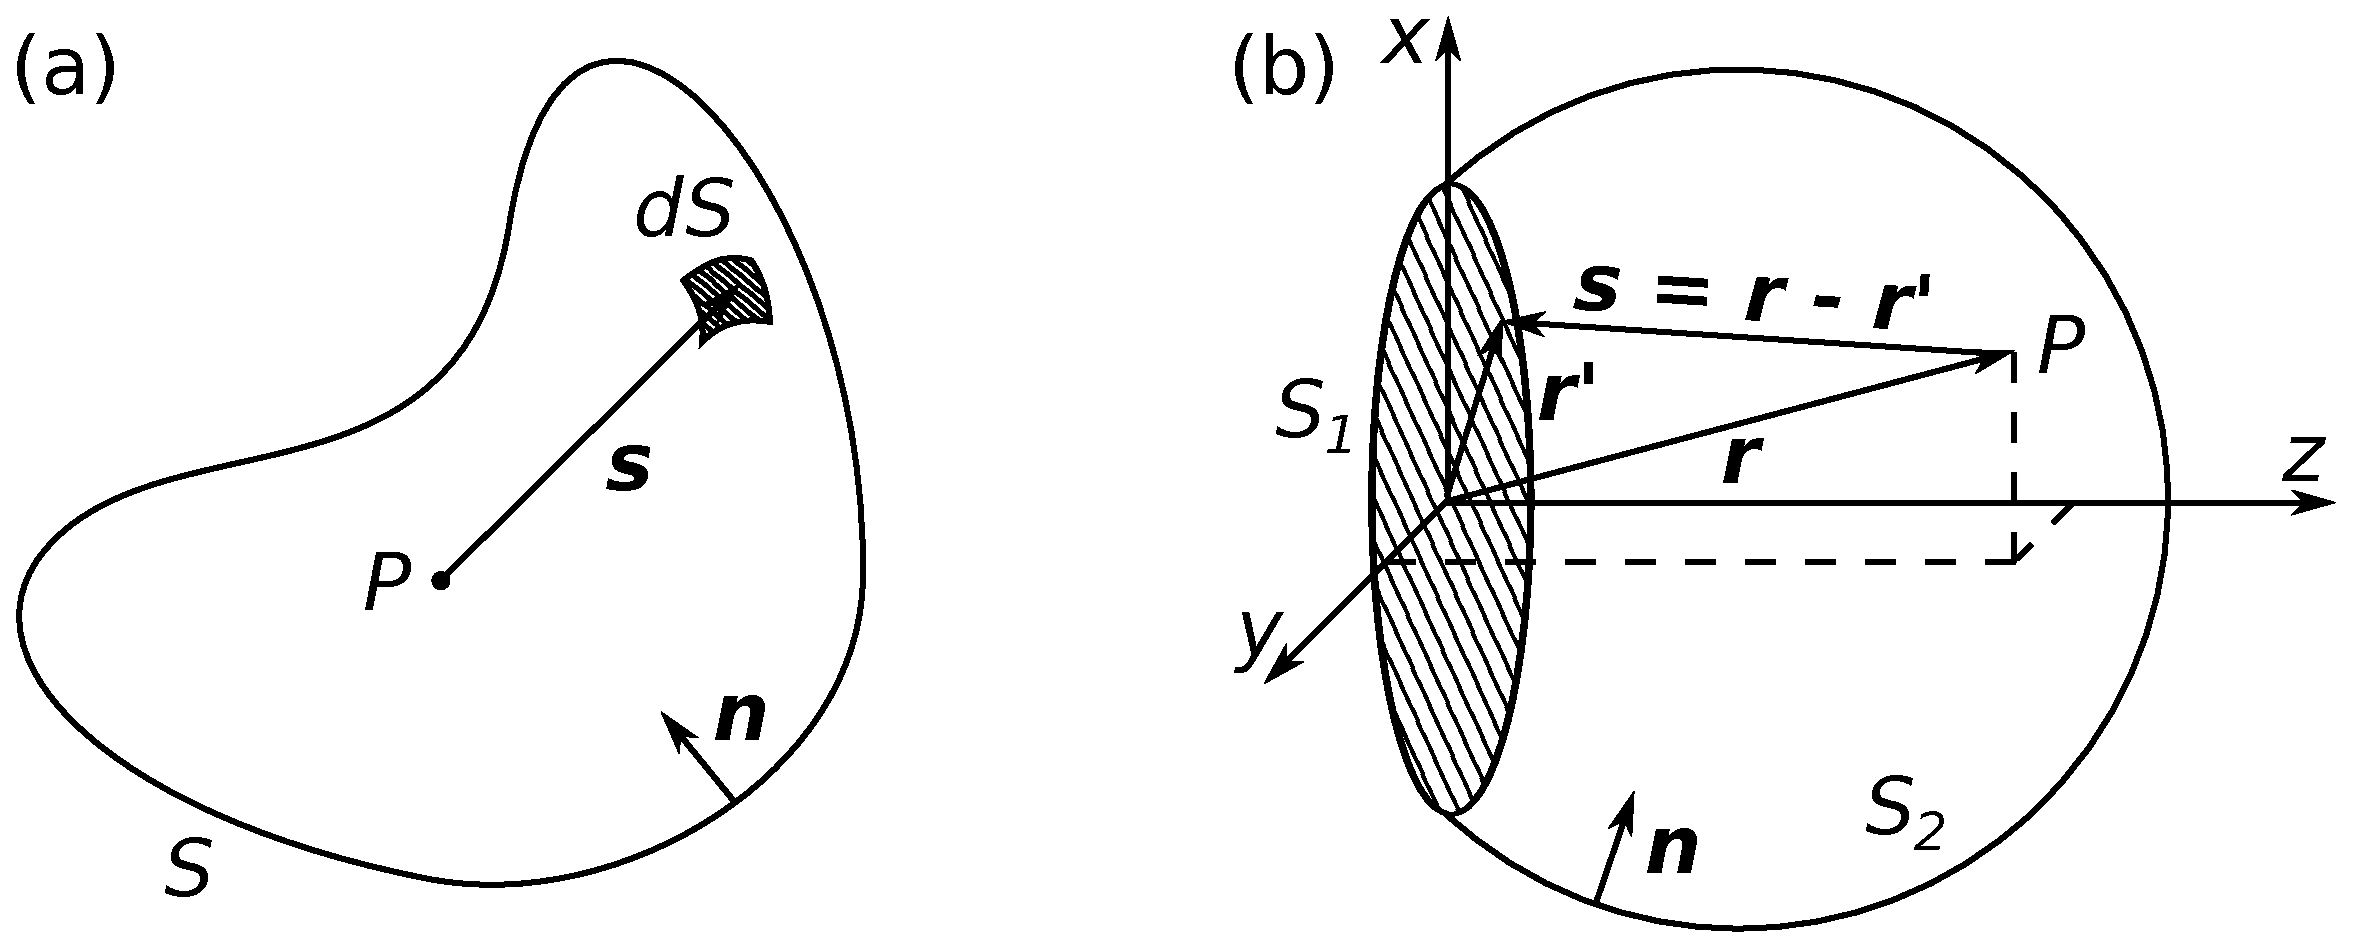
\includegraphics[width = \textwidth]{%
    Chapters/InterferometricMethods/figs/kirchhoff_geometry.eps}
  \caption[Geometries for Kirchhoff diffraction calculations]{%
    Geometries for Kirchhoff diffraction calculations.
    When $S_1$ is imaged by an optical system,
    $S_1$ is referred to as the \emph{object plane}.}
\label{fig:InterferometricMethods:Kirchhoff_geometry}
\end{figure}

To proceed with the diffraction calculation,
assume that the incident waves propagate in the $+z$-direction and
adopt the surface drawn
in Fig.~\ref{fig:InterferometricMethods:Kirchhoff_geometry}(b).
That is, $S = S_1 + S_2$,
where $S_1$ is a circle in the $(x, y)$-plane, and
$S_2$ is a spherical segment centered on the optical axis.
When $S_1$ is imaged by an optical system,
$S_1$ is referred to as the \emph{object plane}.
Now, assume that the incident waves were ``turned on''
at some finite time in the past, and
take the radius of $S_2$ to be large enough such that
none of the diffracted waves have had sufficient time to reach $S_2$,
i.e.\ $U \equiv 0$ on $S_2$.
(Of course, strictly speaking, the source's finite turn-on time
requires relaxation of the monochromatic assumption.
Finite turn-on time does not preclude a pseudo-monochromatic source, however,
and such a source is assumed hereafter).
Thus, the integral over $S_2$ vanishes, and
the diffraction calculation reduces to an integral over $S_1$.

Now, evaluation of
the Helmholtz-Kirchhoff integral
(\ref{eq:InterferometricMethods:Helmholtz_Kirchhoff_integral_theorem})
requires knowledge of $U$ on $S_1$.
For free-space propagation,
$S_1$ is an imagined (rather than a physical) surface
that does not impede the propagation of the incident wave $U^{(i)}$
(that is, $U = U^{(i)}$ and
$\partial U / \partial n = \partial U^{(i)} / \partial n$ on $S_1$).
If, however, $S_1$ contains opaque obstacles,
the free-space propagation conditions are no longer valid;
instead, the Kirchhoff boundary conditions can be adopted:
\begin{align}
  \text{surfaces of clear aperture:}&
  \quad
  U = U^{(i)},
  \quad
  \frac{\partial U}{\partial n} = \frac{\partial U^{(i)}}{\partial n},
  \notag \\
  \text{opaque surfaces:}&
  \quad \;
  U = 0,
  \qquad
  \frac{\partial U}{\partial n} = 0.
  \notag
\end{align}
While these boundary conditions are adequate for the current application,
it should be noted that they are not physical
for points that are very close to the boundaries of the opaque obstacles.


\subsection{Fraunhofer diffraction of a free-space Gaussian beam}
This section demonstrates that the Fraunhofer diffraction formalism
gives the correct form for a free-space Gaussian beam in the far-field limit,
and it also lays the groundwork for examining
the diffraction of a Gaussian beam from plasma-density fluctuations.

Assume that the incident Gaussian beam has a waist at $S_1$, and
take the radius of $S_1$ to be much larger than the beam waist $w_0$
such that the domain of integration effectively extends
over the whole $(x, y)$-plane.
For free-space propagation,
$S_1$ does not perturb the Gaussian beam; thus,
$E(\vect{r}, t) = E^{(i)}(\vect{r}, t) = E_G(\vect{r}) e^{-i \omega_0 t}$.
Now, in the far-field ($k_0 s \gg 1$) and
paraxial ($\vect{s} \approx -z \hat{\vect{z}}$) approximations
\begin{align}
  \left. \frac{e^{i k_0 s}}{s} \right|_{S_1}
  &\approx
  \frac{e^{i k_0 s}}{z},
  \notag \\
  \left. \frac{\partial}{\partial n}
  \left( \frac{e^{i k_0 s}}{s} \right) \right|_{S_1}
  &\approx
  -i k_0 \left( \frac{e^{i k_0 s}}{z} \right).
  \notag
\end{align}
The $s$-dependence in the phase arguments has been retained,
as it is the mechanism responsible for diffraction, but
the $s$-dependence in the amplitude has been dropped
as it only gives rise to negligible variations
in the amplitude of the diffracted wave.
Relative to a spherical wave,
a Gaussian beam has several additional $z$-dependencies;
however, at the beam's waist
\begin{align}
  \left. \frac{\partial w(z)}{\partial z} \right|_{\text{waist}}
  &\equiv
  0,
  \notag \\
  \left. \frac{\partial}{\partial z}
  \left[ \frac{1}{R(z)} \right] \right|_{\text{waist}}
  &=
  \frac{1}{z_R^2},
  \notag \\
  \left. \frac{\partial \psi(z)}{\partial z} \right|_{\text{waist}}
  &=
  \frac{1}{z_R}.
  \notag
\end{align}
Then, if the beam's Rayleigh range is much greater than
the probe wavelength ($k_0 z_R \gg 1$) and
the relevant transverse dimensions are much less than
the Rayleigh range ($w_0 \ll z_R$),
the Gaussian beam at $S_1$ satisfies
\begin{align}
  \left. E_G(\vect{r}') \right|_{S_1}
  &\approx
  E_0 e^{-(\rho' / w_0)^2},
  \notag \\
  \left. \frac{\partial E_G(\vect{r}')}{\partial n} \right|_{S_1}
  &\approx
  i k_0 \left[ E_0 e^{-(\rho' / w_0)^2} \right].
  \notag
\end{align}
Note that the CO$_2$ laser beams ($k_0 \approx \SI{2 \pi e5}{\per\meter}$)
that probe tokamak plasmas often have $z_R \gg \SI{10}{\meter}$
such that $k_0 z_R \gg 1$ and $w_0 \ll z_R$
(the transverse dimensions are constrained by the machine size
such that $w_0 \ll \SI{1}{\meter}$) are very well-satisfied.

Substituting the above expressions for
the incident waves and their surface-normal derivatives into
the Helmholtz-Kirchhoff integral
(\ref{eq:InterferometricMethods:Helmholtz_Kirchhoff_integral_theorem})
and simplifying yields
\begin{equation}
  E(\vect{r})
  \approx
  \frac{-i E_0}{\lambda_0 z}
  \int_{S_1}
  e^{-( \rho' / w_0 )^2}
  e^{i k_0 s}
  dS.
  \label{eq:InterferometricMethods:Kirchhoff_diffraction_integral}
\end{equation}
To proceed further, $s$ must be approximated:
\begin{align}
  s
  &=
  | \vect{\rho}' - \vect{r}|
  \notag \\
  &=
  \left[ r^2 - 2(x'x + y'y) + (x'^2 + y'^2) \right]^{1/2}
  \notag \\
  &\approx
  r - \frac{x'x + y'y}{r},
  \label{eq:InterferometricMethods:Fraunhofer_s}
\end{align}
where only terms linear in $(x' / r)$ and $(y' / r)$ have been retained.
This is known as the Fraunhofer limit, and
it is valid in the far-field $z \gg z_R$~\cite[Sec.~8.3.3]{born_and_wolf}.
Under the Fraunhofer limit
the diffraction integral
(\ref{eq:InterferometricMethods:Kirchhoff_diffraction_integral}) becomes
\begin{equation}
  E(\vect{r})
  \approx
  \frac{-i E_0}{\lambda_0 z}
  e^{i k_0 r}
  D_x D_y,
  \label{eq:InterferometricMethods:Fraunhofer_diffracted_field}
\end{equation}
where
\begin{align}
  D_x
  &=
  \int_{-\infty}^{\infty}
  e^{-( x' / w_0 )^2}
  e^{-i k_0 x' x / r}
  dx'
  \label{eq:InterferometricMethods:Fraunhofer_diffraction_integral_free_space}
  \\
  &=
  \mathcal{F} \left[%
    e^{-( x' / w_0 )^2}
  \right](k_0 x / r)
  \notag \\
  &=
  \sqrt{\pi} w_0 e^{-(k_0 w_0 x / 2 r)^2}
  \label{eq:InterferometricMethods:Fourier_transform_free_space_Gaussian}
\end{align}
gives the diffraction pattern in the $x$-direction, and
the integral has been easily evaluated by noting that
it is simply the Fourier transform of a Gaussian.
The diffraction pattern in the $y$-direction, $D_y$, is similarly determined.
Note that the $e^{-i k_0 x' x / r} = e^{-i k_0 x' \sin\theta}$ term in
(\ref{eq:InterferometricMethods:Fraunhofer_diffraction_integral_free_space})
is the typical geometric phase factor
that results from path-length differences between
points on surface $S_1$ and the field point $\vect{r}$, as shown in
Fig.~{\ref{fig:InterferometricMethods:Fraunhofer_geometric_phase_factor}}.
Substituting
(\ref{eq:InterferometricMethods:Fourier_transform_free_space_Gaussian}) into
(\ref{eq:InterferometricMethods:Fraunhofer_diffracted_field}) yields
\begin{equation}
  E(\vect{r})
  \approx
  -i E_0
  \left( \frac{z_R}{z} \right)
  e^{-(k_0 w_0 \rho / 2 r)^2}
  e^{i k_0 r}.
  \label{eq:InterferometricMethods:Fraunhofer_Gaussian_beam_diffraction}
\end{equation}
Is this consistent
with the expected far-field representation of a Gaussian beam? Yes!
To see this, note that in the far-field ($z \gg z_R$)
\begin{align}
  \frac{z_R}{z}
  &\approx
  \frac{w_0}{w(z)},
  \notag \\
  \frac{k_0 w_0 \rho}{2 r}
  &\approx
  \frac{\rho}{w(z)},
  \notag \\
  r
  &\approx
  z + \frac{\rho^2}{2 R(z)},
  \notag \\
  -i
  = e^{-i \pi / 2}
  &\approx
  e^{-i \psi(z)},
  \notag
\end{align}
such that the diffracted field in the Fraunhofer limit
(\ref{eq:InterferometricMethods:Fraunhofer_Gaussian_beam_diffraction})
can be cast in the form of a typical Gaussian beam
as expressed in
(\ref{eq:InterferometricMethods:Gaussian_beam}),
i.e.\ $E(\vect{r}) = E_G(\vect{r})$ for $z \gg z_R$.
Of course, when considering free-space propagation,
$E(\vect{r}) \equiv E_G(\vect{r})$ for $0 \leq z < \infty$, but
the above work \emph{proves} that
the Fraunhofer diffraction formalism
gives the correct results under the appropriate limits;
it also lays the groundwork for examining
the diffraction of a phase-modulated Gaussian beam.

\begin{figure}
  \centering
  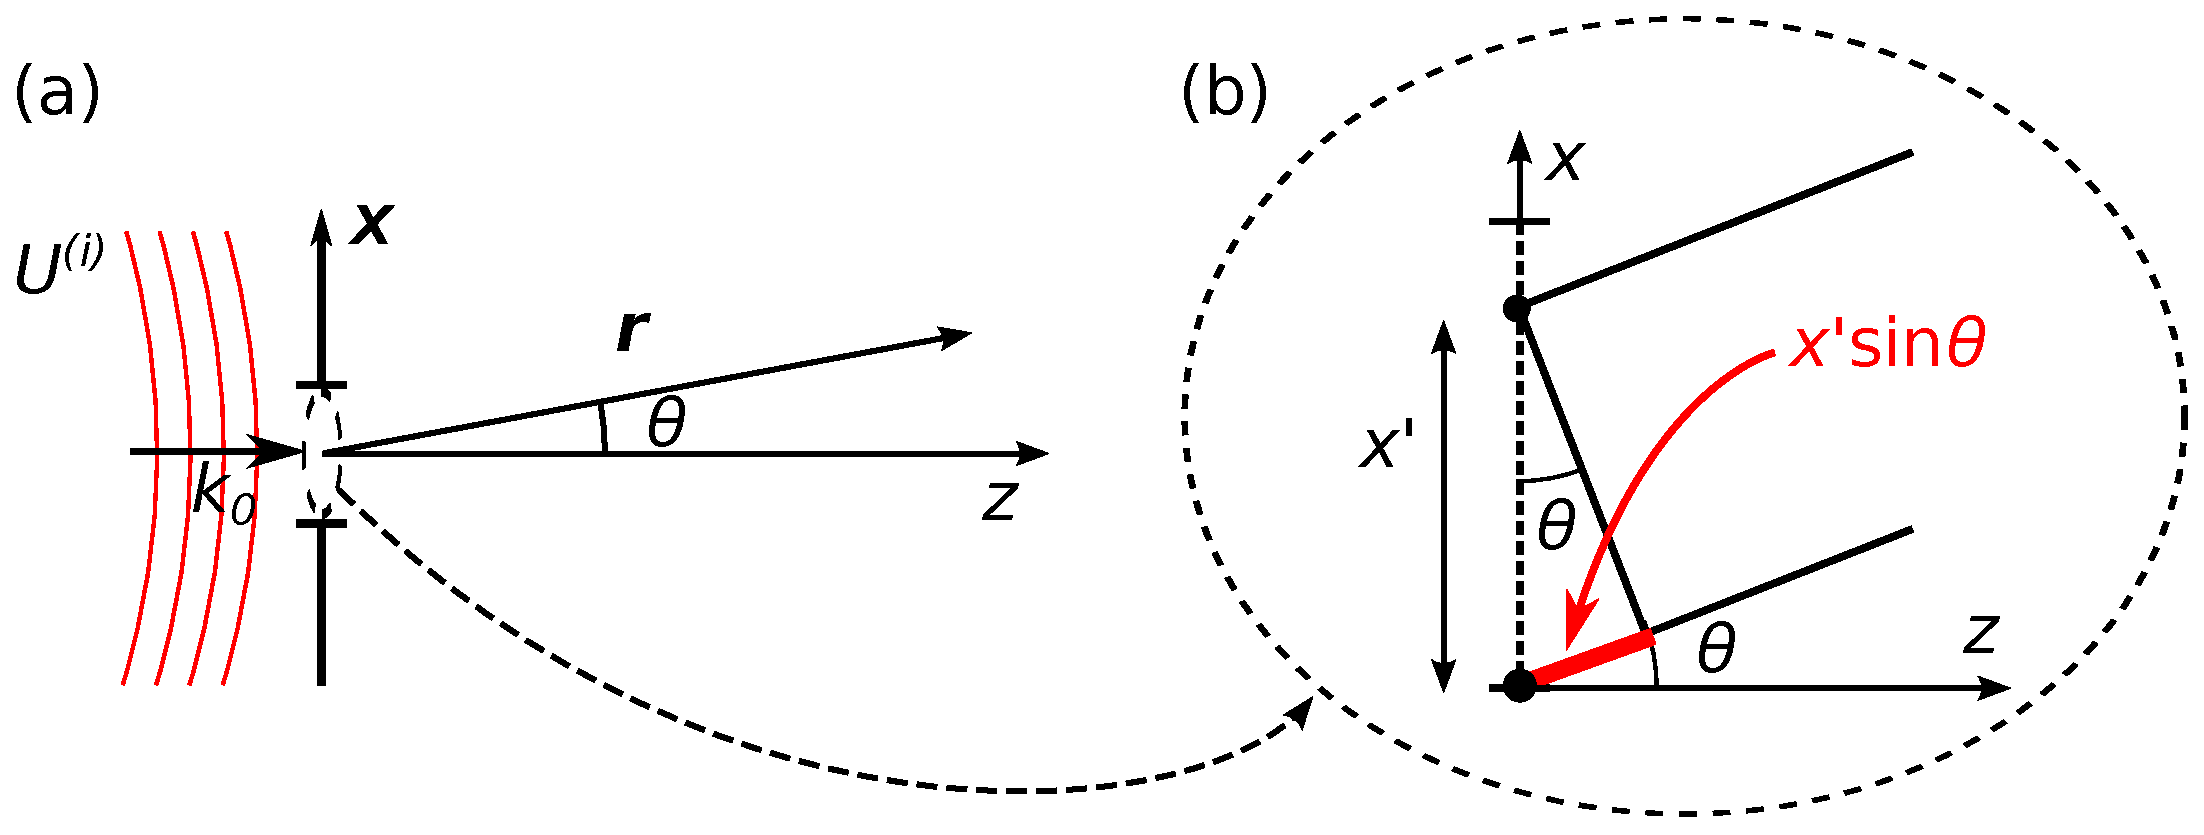
\includegraphics[width = \textwidth]{%
    Chapters/InterferometricMethods/figs/Fraunhofer_geometric_phase_factor.eps}
  \caption[Fraunhofer geometric phase factor]{%
    (a) Typical Fraunhofer diffraction geometry and
    (b) a close up that displays the path-length difference $x' \sin\theta$
    between a wave emanating from the origin and
    a wave emanating from $x'$}
\label{fig:InterferometricMethods:Fraunhofer_geometric_phase_factor}
\end{figure}


\subsection{Diffraction of a Gaussian beam from plasma-density fluctuations}
\label{sec:InterferometricMethods:Gaussian_beam_diffraction:from_plasma_density_fluctuations}
Now, allow a Gaussian, CO$_2$ probe beam
to pass through a tokamak plasma.
The beam acquires the plasma-induced phase delay $\phi(\vect{\rho}', t)$
given by (\ref{eq:InterferometricMethods:phase}),
where $\vect{\rho}'$ corresponds to the beam's transverse dimensions.
Explicitly dividing $\phi$ into bulk $\bar{\phi}(t)$ and
spatially varying $\tilde{\phi}(\vect{\rho}', t)$ components,
the plasma-induced phase delay becomes
\begin{equation}
  \phi(\vect{\rho}', t) = \bar{\phi}(t) + \tilde{\phi}(\vect{\rho}', t).
\end{equation}
Typically, $\tilde{\phi}$ varies on much faster time scales than $\bar{\phi}$,
but this is not required.
The spatial variation of the plasma-induced phase delay
contributes to the diffraction of the incident Gaussian probe beam, and
the remainder of this section uses scalar-diffraction theory
to determine the diffracted field in the Fraunhofer limit;
the near-field form consistent with the computed Fraunhofer field
is then inferred.
(The object planes of the imaging systems relevant to this work
sit in the near field, so computation of the imaged field requires
knowledge of the near-field diffraction pattern).

The response functions of the diagnostics investigated in
Sections~\ref{sec:InterferometricMethods:interferometry} and
\ref{sec:InterferometricMethods:pci} will be shown
to be linear in their regimes of relevance, so
it is sufficient to examine phase fluctuations $\tilde{\phi}$
consisting of a single Fourier mode
\begin{equation}
  \tilde{\phi}(\vect{\rho}', t) = \tilde{\phi}_0 \cos(k x' - \omega t).
  \label{eq:InterferometricMethods:cosine_phase_fluctuation}
\end{equation}
As a CO$_2$ beam's optical cycles
($\omega_0 = 2 \pi \cdot \SI{28.3}{\tera\hertz}$)
occur much more rapidly than the temporal evolution of the plasma
($\omega \lesssim 2 \pi \cdot \SI{1}{\giga\hertz}$),
the problem can be treated adiabatically
by solving for the beam propagation
at each instant in time during the relatively slow evolution of $\phi$.
Then, following the formalism pioneered by Raman and Nath
\cite{raman_nath_diffraction_partI,raman_nath_diffraction_partIII},
this plasma-induced phase delay makes an additional phase contribution
to the diffraction integral
(\ref{eq:InterferometricMethods:Fraunhofer_diffraction_integral_free_space})
such that the diffraction pattern in the $x$-direction is given as
\begin{align}
  D_x
  &=
  \int_{-\infty}^{\infty}
  e^{-( x' / w_0 )^2}
  e^{-i k_0 x x' / r}
  e^{i \phi(x', t)}
  dx'
  \notag \\
  &=
  e^{i \bar{\phi}}
  \int_{-\infty}^{\infty}
  e^{-( x' / w_0 )^2}
  e^{-i k_0 x x' / r}
  e^{i \tilde{\phi}_0 \cos(k x' - \omega t)}
  dx'
  \notag \\
  &\begin{aligned}
    =
    e^{i \bar{\phi}}
    &\int_{-\infty}^{\infty}
    e^{-( x' / w_0 )^2}
    e^{-i k_0 x x' / r}
    \\
    &\times
    \left\{%
      \sum_{m = -\infty}^{\infty}
      i^m \left[ J_m(\tilde{\phi}_0) \right]
      e^{i m (k x' - \omega t)}
    \right\}
    dx'
  \end{aligned}
  \notag \\
  &\begin{aligned}
    =
    e^{i \bar{\phi}}
    &\sum_{m = -\infty}^{\infty}
    i^m \left[ J_m(\tilde{\phi}_0) \right]
    e^{-i m \omega t}
    \\
    &\times
    \int_{-\infty}^{\infty}
    e^{-( x' / w_0 )^2}
    e^{-i \left( \frac{k_0 x}{r} - m k \right) x'}
    dx'
  \end{aligned}
  \notag \\
  &\begin{aligned}
    =
    \sqrt{\pi} w_0
    e^{i \bar{\phi}}
    \sum_{m = -\infty}^{\infty}
    \biggl\{
      &i^m \left[ J_m(\tilde{\phi}_0) \right]
      e^{-i m \omega t}
      \\
      &\qquad \times
      e^{-\left[ \frac{w_0}{2} \left( \frac{k_0 x}{r} - m k \right) \right]^2}
    \biggr\},
  \end{aligned}
  \label{eq:InterferometricMethods:Fraunhofer_diffraction_integral_phase_modulated}
\end{align}
where the bracketed expression in the third equality follows from
application of the well-known Jacobi-Anger expansion and
$J_m$ is the $m$\ts{th} Bessel function of the first kind.
Noting that $E(\vect{r}, t) = E(\vect{r}) e^{-i \omega_0 t}$,
substitution of
(\ref{eq:InterferometricMethods:Fraunhofer_diffraction_integral_phase_modulated})
into (\ref{eq:InterferometricMethods:Fraunhofer_diffracted_field}) yields
\begin{align}
  \begin{aligned}
    E(\vect{r}, t)
    \approx
    &\sum_{m = -1}^{1}
    i^m \left[ J_m(\tilde{\phi}_0) \right]
    e^{-i m \omega t}
    e^{-\left[ \frac{w_0}{2} \left( \frac{k_0 x}{r} - m k \right) \right]^2}
    \\
    &\times
    e^{i \bar{\phi}}
    \left[
      -i E_0
      \left( \frac{z_R}{z} \right)
      e^{-(k_0 w_0 y / 2 r)^2}
      e^{i (k_0 r - \omega_0 t)}
    \right].
  \label{eq:InterferometricMethods:Fraunhofer_phase_modulated_Gaussian_beam_diffraction}
  \end{aligned}
\end{align}
Here, only the $|m| \leq 1$ terms have been retained because
$|J_m(\tilde{\phi}_0)| \sim \tilde{\phi}_0^{|m|}$
for experimentally relevant values of $\tilde{\phi}_0 \ll 1$.
(The complete small-argument, asymptotic form for $J_m$ is discussed in
Section~\ref{sec:InterferometricMethods:imaging:weak_coupling_limit}).
The effect of higher order terms can be easily investigated
by e.g.\ including the $m = \pm 2$ terms etc.

\begin{figure}
  \centering
  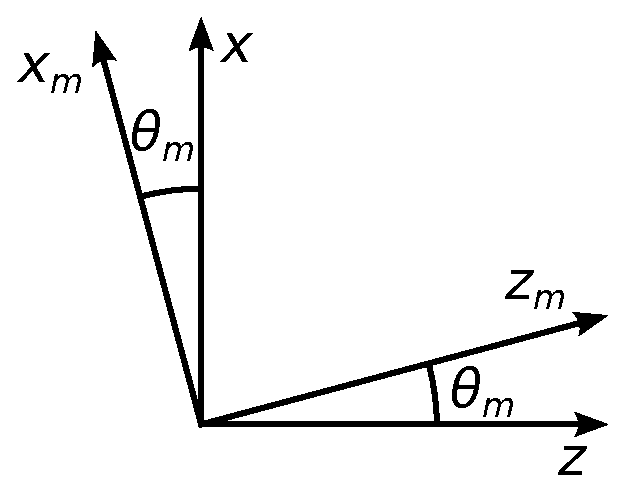
\includegraphics[width = 0.4 \textwidth]{%
    Chapters/InterferometricMethods/figs/coordinate_rotation.eps}
  \caption{Coordinate transformation for interpretation of
    the diffraction pattern of a phase-modulated Gaussian beam}
\label{fig:InterferometricMethods:coordinate_rotation}
\end{figure}

To put
(\ref{eq:InterferometricMethods:Fraunhofer_phase_modulated_Gaussian_beam_diffraction})
in a more familiar form,
consider the coordinate transformation
from the lab-frame coordinate system $\vect{r}$
to the coordinate system of the $m$\ts{th} scattered beam $\vect{r}_m$,
as depicted graphically
in Fig.~\ref{fig:InterferometricMethods:coordinate_rotation}.
As the transformation is simply
a rotation about the $y$-axis by angle $\theta_m$,
the coordinate systems are related via
\begin{equation}
  \begin{pmatrix}
    x_m
    \\
    y_m
    \\
    z_m
  \end{pmatrix}
  =
  \begin{pmatrix}
    \cos\theta_m & 0 & -\sin\theta_m
    \\
    0            & 1 & 0
    \\
    \sin\theta_m & 0 & \cos\theta_m
  \end{pmatrix}
  \begin{pmatrix}
    x
    \\
    y
    \\
    z
  \end{pmatrix},
  \label{eq:InterferometricMethods:object_plane_coordinate_transformation_explicit}
\end{equation}
where
\begin{equation}
  \sin \theta_m
  \equiv
  \frac{m k}{k_0}.
  \label{eq:InterferometricMethods:scattering_angles}
\end{equation}
Typically, $m k / k_0 \ll 1$ such that
\begin{equation}
  \cos \theta_m
  \approx
  1 - \frac{1}{2} \left( \frac{m k}{k_0} \right)^2
\end{equation}
is a very good approximation.
The above coordinate transformation can be written more compactly as
\begin{equation}
  \vect{r}_m
  =
  [ \vect{R}(\theta_m) ] \vect{r},
  \label{eq:InterferometricMethods:object_plane_coordinate_transformation_compact}
\end{equation}
where
\begin{equation}
  \vect{R}(\theta)
  =
  \begin{pmatrix}
    \cos\theta & 0 & -\sin\theta
    \\
    0          & 1 & 0
    \\
    \sin\theta & 0 & \cos\theta
  \end{pmatrix}
  \label{eq:InterferometricMethods:rotation_matrix}
\end{equation}
is the rotation matrix
that rotates the $(x, z)$-plane about the $y$-axis by angle $\theta$.
Rotation matrices are \emph{orthogonal},
which endows $\vect{R}(\theta_m)$ with some useful properties
\cite[Ch.~6]{FB_linear_algebra};
namely, its inverse is equal to its transpose $[\vect{R}(\theta_m)]^T$
\begin{equation}
  [\vect{R}(\theta_m)]^T
  =
  [\vect{R}(\theta_m)]^{-1}
  =
  \vect{R}(-\theta_m),
  \label{eq:InterferometricMethods:rotation_matrix_inverse_relationships}
\end{equation}
and its determinant is unity
\begin{equation}
  \text{det}[\vect{R}(\theta_m)] = |\vect{R}(\theta_m)| = 1
  \label{eq:InterferometricMethods:rotation_matrix_determinant}
\end{equation}
such that the rotation preserves lengths, i.e.\ $r_m = r$.
It is sufficient to retain terms only to first order in
$k / k_0$ (small scattering angle) and $x / z$ (paraxial limit)
for the \emph{amplitude} dependencies of the diffracted field
(this is \emph{not}, in general, true for the phase dependencies).
Thus, $1 / z \approx 1 / z_m$ and $x \approx x_m + (m k / k_0) z$
such that the Fraunhofer diffracted field
(\ref{eq:InterferometricMethods:Fraunhofer_phase_modulated_Gaussian_beam_diffraction})
can be rewritten as
\begin{equation}
  \begin{aligned}
    E(\vect{r}, t)
    \approx
    e^{i \bar{\phi}}
    &\sum_{m = -1}^{1}
    i^m \left[ J_m(\tilde{\phi}_0) \right]
    e^{-i (\omega_0 + m \omega) t}
    \\
    &\times
    \left[
      -i E_0
      \left( \frac{z_R}{z_m} \right)
      e^{-(k_0 w_0 \rho_m / 2 r)^2}
      e^{i k_0 r}
    \right],
  \end{aligned}
\end{equation}
where $\rho_m = (x_m^2 + y_m^2)^{1/2}$.
Now, the bracketed expression has the form of
(\ref{eq:InterferometricMethods:Fraunhofer_Gaussian_beam_diffraction})
for a far-field Gaussian beam; thus,
the diffracted electric field can be more compactly and generally written as
\begin{equation}
  E(\vect{r}, t)
  \approx
  e^{i \bar{\phi}}
  \sum_{m = -1}^{1}
  i^m \left[ J_m(\tilde{\phi}_0) \right]
  E_G(\vect{r}_m)
  e^{-i (\omega_0 + m \omega) t}.
  \label{eq:InterferometricMethods:phase_modulated_Gaussian_beam_diffraction}
\end{equation}
Note that
(\ref{eq:InterferometricMethods:phase_modulated_Gaussian_beam_diffraction})
is valid for $0 \leq z < \infty$ rather than only for $z \gg z_R$;
that is, computing the far-field diffraction pattern
has additionally allowed \emph{inferring} the corresponding near field.

Thus, a sinusoidal phase modulation diffracts an incident Gaussian beam
predominantly into downscattered ($m = -1$), unscattered ($m = 0$), and
upscattered ($m = 1$) Gaussian beams.
The incident beam is coupled into the $m$\ts{th} scattered beam
with strength $J_m(\tilde{\phi}_0)$.
The $m$\ts{th} scattered beam is Doppler shifted
relative to the incident beam by $m \omega$ and
propagates at an angle $\theta_m \approx m k / k_0$
relative to the lab-frame optical axis.
The adiabatic assumption ($\omega / \omega_0 \ll 1$)
is very well-satisfied for a CO$_2$ probe beam
in a typical tokamak plasma
(i.e.\
$\omega / \omega_0
\lesssim
\SI{1}{\giga\hertz} / \SI{28.3}{\tera\hertz}
\sim 10^{-5}$).
Thus, the scattering is very nearly elastic, and
$|\vect{k}_{0,m}| = k_0$ is a very good approximation.
This constraint of elasticity
coupled with knowledge of the scattering angle $\theta_m$
allows determination of the scattered wavevector
\begin{equation}
  \vect{k}_{0,m}
  =
  (m k) \hat{\vect{x}}
  +
  k_0 \left[ 1 - \left(\frac{m k}{k_0}\right)^2 \right]^{1/2} \hat{\vect{z}}.
  %k_0 \sqrt{1 - \left(\frac{m k}{k_0}\right)^2} \hat{\vect{z}}
  \label{eq:InterferometricMethods:scattered_beam_wavevector}
\end{equation}
Finally, note that the simultaneous presence
of both the upscattered and downscattered beams
under typical experimental conditions
has been demonstrated empirically
\cite[Sec.~2.1]{dorris_phd}.
In the above formalism, the simultaneous upscattering and downscattering
of the incident probe beam results from
the assumption of a sinusoidal phase fluctuation in
(\ref{eq:InterferometricMethods:cosine_phase_fluctuation});
if a complex exponential were assumed instead,
one would erroneously deduce that
only one such scattering process (either up or down) occurs.


\subsection{Validity of the Raman-Nath formalism}
The Raman-Nath formalism employed in
Section~\ref{sec:InterferometricMethods:Gaussian_beam_diffraction:from_plasma_density_fluctuations}
is valid as long as the fluctuation wavenumber $k$ is not too large.
This constraint has been rigorously quantified by Bhatia and Noble
\cite{bhatia_53_general_theory,bhatia_53_approximate_expressions_for_intensities} and
is also discussed by Born and Wolf
\cite[Ch.~12]{born_and_wolf}.
Specifically, beam diffraction will be in the Raman-Nath regime when
\begin{equation}
  \delta = \frac{\tilde{n}_e}{\bar{n}_e} \left( \frac{k_0}{k} \right)^2 \gg 1,
  \label{eq:InterferometricMethods:raman_nath_validity_criterion}
\end{equation}
where
$\bar{n}_e$ is the bulk plasma density,
$\tilde{n}_e$ is the amplitude of the plasma-density fluctuation,
$k_0$ is the vacuum wavenumber of the probe beam, and
$k$ is the wavenumber of the plasma-density fluctuation.
Note that the above $\delta$ is equivalent
to that used by Bhatia and Noble,
after having made the appropriate substitutions
for a CO$_2$ probe beam in a tokamak plasma.
Assuming typical tokamak values
\begin{align}
  &\frac{\tilde{n}_e}{\bar{n}_e}
  \sim
  10^{-3},
  \notag \\
  &k
  \lesssim
  \SI{30}{\per\centi\meter}
  \notag
\end{align}
yields $\delta \gtrsim 40$
for a CO$_2$ probe beam ($k_0 \approx 2 \pi \cdot \SI{e5}{\per\meter}$)
such that beam's diffraction is well within the Raman-Nath regime.
In the opposite regime ($\delta \ll 1$)
the beam can \emph{Bragg scatter} from the phase fluctuation,
producing a single, strongly-scattered beam
\cite{bhatia_53_approximate_expressions_for_intensities}
\cite[Ch.~12]{born_and_wolf};
such Bragg scattering is the foundation of acousto-optics.


\subsection{Wavenumber-dependent manipulation of the diffracted field}
Examine again the diffracted field
(\ref{eq:InterferometricMethods:phase_modulated_Gaussian_beam_diffraction}).
The spatial dependence of each term in the summation
is wholly governed by the factor $E_G(\vect{r}_m)$,
which corresponds to a Gaussian beam
that emanates from the beam waist
at an angle $\theta_m$ relative to the lab-frame $z$-axis.
The coordinate system $\vect{r}_m$ is defined such that
the $m$\ts{th} Gaussian beam propagates along the $z_m$-axis, and
it is related to the lab-frame coordinate system $\vect{r}$ via
(\ref{eq:InterferometricMethods:object_plane_coordinate_transformation_compact}).
The wavenumber basis $\vect{k}_m$ that is dual to $\vect{r}_m$
is similarly related to the lab-frame wavenumber basis $\vect{k}$ via
\begin{equation}
  \vect{k}_m
  =
  [ \vect{R}(\theta_m) ] \vect{k},
  \label{eq:InterferometricMethods:object_plane_coordinate_transformation_wavenumber_dual}
\end{equation}
which naturally results from the geometric constraint that
$\vect{k} \cdot \vect{r} = \vect{k}_m \cdot \vect{r}_m$.

Imagine now that each of the above Gaussian beams
is somehow manipulated based upon its Fourier wavenumber content.
Assume this manipulation can be described
in terms of a transfer function $T(\vect{k})$,
where $\vect{k}$ is the lab-frame wavenumber basis.
A transfer functions of this form is appropriate for investigating e.g.\
diffraction from an aperture or the action of a phase plate.
Using the wavenumber basis transformation
(\ref{eq:InterferometricMethods:object_plane_coordinate_transformation_wavenumber_dual}),
this transfer function can be written
in terms of the $\vect{k}_m$ wavenumber basis as
\begin{equation}
  T(\vect{k}) = T(\vect{R}_{-m} \vect{k}_m),
\end{equation}
where the abbreviation $\vect{R}_m = \vect{R}(\theta_m)$ has been adopted.
The transformed field $E_T$ then has the Fourier representation
in the $\vect{k}_m$ wavenumber basis
\begin{equation}
  E_T(\vect{k}_m) = T(\vect{R}_{-m} \vect{k}_m) \cdot E_G(\vect{k}_m).
\end{equation}
Inverse Fourier transforming $E_T(\vect{k}_m)$ yields
\begin{equation}
  E_T(\vect{r}_m)
  =
  \frac{1}{(2 \pi)^3}
  \int d\vect{k}_m \,
  \left[%
    T(\vect{R}_{-m} \vect{k}_m)
    e^{i \vect{k}_m \cdot \vect{r}_m}
  \right]
  E_G(\vect{k}_m).
\end{equation}
Note that each spectral component $E_G(\vect{k}_m)$
individually satisfies the wave equation.
Thus, the above construction of the transformed field $E_T(\vect{r}_m)$,
which consists of a linear combination of the spectral components
with arbitrary amplitudes and phases,
\emph{also} satisfies the wave equation.
Now, explicitly writing $E_G(\vect{k}_m)$ as the Fourier transform
of $E_G$ over a dummy spatial coordinate $\vect{r}'$, and
exchanging the order of integration yields
\begin{equation}
  E_T(\vect{r}_m)
  =
  \frac{1}{(2 \pi)^3}
  \int d\vect{r}' \,
  E_G(\vect{r}')
  \int d\vect{k}_m \,
  T(\vect{R}_{-m} \vect{k}_m)
  e^{i \vect{k}_m \cdot (\vect{r}_m - \vect{r}')}.
\end{equation}
Further, for the applications considered here,
it is advantageous to change the variables of integration
from the $\vect{k}_m$ wavenumber basis
to the lab-frame wavenumber basis $\vect{k}$.
Note that
\begin{equation}
  d\vect{k}_m
  =
  \left| \frac{\partial \vect{k}_m}{\partial \vect{k}} \right|
  d\vect{k}
  =
  |\vect{R}_m|
  d\vect{k}
  =
  d\vect{k}
\end{equation}
and that
\begin{align}
  \vect{k}_m \cdot (\vect{r}_m - \vect{r}')
  &=
  (\vect{R}_m \vect{k}) \cdot (\vect{r}_m - \vect{r}')
  \notag \\
  &=
  (\vect{R}_m \vect{k})^T (\vect{r}_m - \vect{r}')
  \notag \\
  &=
  \vect{k}^T \vect{R}_m^T (\vect{r}_m - \vect{r}')
  \notag \\
  &=
  \vect{k} \cdot [\vect{R}_{-m} (\vect{r}_m - \vect{r}')]
\end{align}
such that the transformed field $E_T(\vect{r}_m)$ becomes
\begin{equation}
  E_T(\vect{r}_m)
  =
  \frac{1}{(2 \pi)^3}
  \int d\vect{r}' \,
  E_G(\vect{r}')
  \int d\vect{k} \,
  T(\vect{k})
  e^{i \vect{k} \cdot \left[ \vect{R}_{-m} (\vect{r}_m - \vect{r}') \right]},
  \label{eq:InterferometricMethods:mth_diffracted_beam_Fourier_filtered}
\end{equation}
where, again, the abbreviation $\vect{R}_{-m} = \vect{R}(-\theta_m)$
has been adopted and $\vect{R}(\theta)$ is the rotation matrix given by
(\ref{eq:InterferometricMethods:rotation_matrix}).

To make further progress,
a particular form of $T(\vect{k})$ is needed.
Assume that wavenumbers are filtered
only in the direction of beam scattering
i.e.\ $T(\vect{k}) = T(k_x)$.
(For example, the groove of a phase plate would be aligned
with the lab-frame $y$-axis to effect such filtering).
Then
\begin{equation}
  \vect{R}_{-m} (\vect{r}_m - \vect{r}')
  =
  \begin{pmatrix}
    (x_m - x') \cos\theta_m + (z_m - z') \sin\theta_m
    \\
    y_m - y'
    \\
    (z_m - z') \cos\theta_m - (x_m - x') \sin\theta_m
  \end{pmatrix}
\end{equation}
such that
(\ref{eq:InterferometricMethods:mth_diffracted_beam_Fourier_filtered})
becomes
\begin{align}
  E_T(\vect{r}_m)
  &=
  \frac{1}{(2 \pi)^3}
  \int d\vect{r}' \,
  E_G(\vect{r}')
  \int dk_y \,
  e^{i k_y (y_m - y')}
  \notag \\
  &\qquad\quad \times
  \int dk_z \,
  e^{i k_z [(z_m - z') \cos\theta_m - (x_m - x') \sin\theta_m]}
  \notag \\
  &\qquad\quad \times
  \int dk_x \,
  T(k_x)
  e^{i k_x \left[ (x_m - x') \cos\theta_m + (z_m - z') \sin\theta_m \right]}
  \notag \\
  &=
  \frac{1}{2 \pi}
  \int d\vect{r}' \,
  E_G(\vect{r}')
  \delta(y_m - y')
  \notag \\
  &\qquad\quad \times
  \delta\bigl( (z_m - z') \cos\theta_m - (x_m - x') \sin\theta_m \bigr)
  \notag \\
  &\qquad\quad \times
  \int dk_x \,
  T(k_x)
  e^{i k_x \left[ (x_m - x') \cos\theta_m + (z_m - z') \sin\theta_m \right]}
  \notag \\
  &\begin{aligned}
    &=
    \frac{1}{2 \pi}
    \int dx' \,
    E_G\bigl( x',\, y_m,\, z_m - (x_m - x')\tan \theta_m \bigr)
    \\
    &\qquad\quad \times
    \int dk_x \,
    T(k_x)
    e^{i k_x (x_m - x') \sec\theta_m}
  \end{aligned}
  \label{eq:InterferometricMethods:mth_diffracted_beam_kx_filtered_v1}
\end{align}
Contributions to the integral from regions outside of $|x'| \lesssim w(z_m)$
are suppressed by the Gaussian envelope such that
\begin{align}
  w\bigl( z_m - (x_m - x')\tan \theta_m \bigr)
  &\approx
  w(z_m),
  \notag \\
  R\bigl( z_m - (x_m - x')\tan \theta_m \bigr)
  &\approx
  R(z_m),
  \notag \\
  \psi\bigl( z_m - (x_m - x')\tan \theta_m \bigr)
  &\approx
  \psi(z_m)
  \notag
\end{align}
are very good approximations.
Note that the phase of the Gaussian beam
\emph{cannot} be approximated in such a manner;
instead, terms up to first order in $\theta_m$
must be retained in the phase.
After making these approximations,
(\ref{eq:InterferometricMethods:mth_diffracted_beam_kx_filtered_v1})
reduces to
\begin{equation}
  E_T(\vect{r}_m)
  \approx
  E_G(0, y_m, z_m)
  \cdot
  \mathcal{E}(\vect{r}_m, k),
  \label{eq:InterferometricMethods:mth_diffracted_beam_kx_filtered_compact}
\end{equation}
where
\begin{equation}
  \begin{aligned}
    \mathcal{E}(\vect{r}_m, k)
    &=
    \frac{e^{-i m k x_m}}{2 \pi}
    \\
    &\quad \times
    \int dx' \,
    \exp\left[ \frac{-x'^2}{w(z_m)^2} \right]
    \exp\left\{%
      i \left[%
        m k x'
        +
        \frac{k_0 x'^2}{2 R(z_m)}
      \right]
    \right\}
    \\
    &\quad \times
    \int dk_x \,
    T(k_x)
    e^{i k_x (x_m - x')}
  \end{aligned}
  \label{eq:InterferometricMethods:mth_diffracted_beam_kx_filtered_transformation}
\end{equation}
is a complex-valued function
that describes the amplitude and phase transformations
that result from filtering the scattered radiation by $T(k_x)$.
(Note that
(\ref{eq:InterferometricMethods:mth_diffracted_beam_kx_filtered_compact})
readily reduces to $E_T(\vect{r}_m) = E_G(\vect{r}_m)$ when $T(k_x) = 1$,
in agreement with expectations).
Generalizing
(\ref{eq:InterferometricMethods:phase_modulated_Gaussian_beam_diffraction})
to allow for such wavenumber-dependent manipulation
yields a total diffracted electric field
\begin{equation}
  E(\vect{r}, t)
  \approx
  e^{i \bar{\phi}}
  \sum_{m = -1}^{1}
  i^m \left[ J_m(\tilde{\phi}_0) \right]
  E_T(\vect{r}_m)
  e^{-i (\omega_0 + m \omega) t}.
  \label{eq:InterferometricMethods:phase_modulated_Gaussian_beam_diffraction_Fourier_filtered}
\end{equation}
Manipulating the total diffracted electric field in such a manner
forms the foundation of phase contrast imaging (PCI),
as will be demonstrated in Section~\ref{sec:InterferometricMethods:pci}.


\section{Imaging of the diffracted field}
\label{sec:InterferometricMethods:imaging}
It is often desirable to \emph{image} the above diffracted field
in order to determine the spatiotemporal aspects
of the responsible phase fluctuations.
Below, the geometric optics and Gaussian beam propagation
of relevance to imaging systems is briefly reviewed
prior to computing the imaged field.


\subsection{The geometric optics of an imaging system}
Let the optical axis of an arbitrary optical system lie along the $z$-axis,
and let all optical rays lie in a plane with the optical axis.
At a given position $z_j$, an optical ray is fully described by
its transverse distance $\rho$ to the optical axis and
its slope $d\rho / dz$.
In the paraxial limit $d\rho / dz \approx \theta$
where $\theta$ is the angle between the ray and the optical axis.
Ray propagation through homogeneous media and refractive interfaces
are well-governed by the so-called $ABCD$ ray matrix formalism
\cite[Ch.~15]{siegman_lasers};
that is, a ray propagating from point $j$ to point $j + 1$ evolves as
\begin{equation}
  \begin{pmatrix}
    \rho_{j + 1}
    \\
    \theta_{j + 1}
  \end{pmatrix}
  =
  \begin{pmatrix}
    A & B
    \\
    C & D
  \end{pmatrix}
  \begin{pmatrix}
    \rho_j
    \\
    \theta_j
  \end{pmatrix},
  \label{eq:InterferometricMethods:ABCD_ray_tracing_general}
\end{equation}
where the $ABCD$ matrix elements are determined
by the optical properties of the media between points $j$ and $j + 1$.
Some rudimentary $ABCD$ matrices are given in
Table~\ref{table:InterferometricMethods:ABCD_matrices}, while
more exhaustive lists can be readily found elsewhere
\cite[Ch.~15]{siegman_lasers}~\cite{tovar_generalized_beam_matrices_IV}.

\begin{table}
  \centering
  \renewcommand{\arraystretch}{1.5}% Spread rows out...
  \begin{tabular}{%
    >{\centering}m{6cm} >{\centering}m{4.5cm}
  }
    \toprule%
    \textbf{optical element} & $\mathbf{ABCD}$~\textbf{matrix}
    \tabularnewline%
    \midrule
    \textbf{propagation} by distance $d$ \\
    through medium of constant \\
    index of refraction, $N$
    &
    $\begin{pmatrix}
      1 & d
      \\
      \phantom{-} 0 \phantom{f} & 1  % phantoms to match thin lens format
    \end{pmatrix}$
    \tabularnewline%
    \textbf{thin lens} with \\
    focal length $f$
    &
    $\begin{pmatrix}
      1 & 0
      \\
      -1/f & 1
    \end{pmatrix}$
    \tabularnewline%
    \toprule%
  \end{tabular}
  \caption[Useful $ABCD$ ray matrices]{Useful $ABCD$ ray matrices.}
\label{table:InterferometricMethods:ABCD_matrices}
\end{table}

An imaging system $\image$, by definition,
redirects all rays emanating from transverse position $\rho_{\object}$
in the object plane $S_{\object}$
to intersect at transverse position
\begin{equation}
  \rho_{\image} = M \rho_{\object}
  \label{eq:InterferometricMethods:image_plane_transverse_coordinates}
\end{equation}
in the image plane $S_{\image}$.
Here, $M$ is the \emph{magnification} of the imaging system, and
$M < 0$ implies that the image is inverted relative to the object.
The imaging system's $A$, $B$, and $D$ matrix elements
are easily determined by inspection.
Recalling the ray-matrix definitions in
(\ref{eq:InterferometricMethods:ABCD_ray_tracing_general}),
note that
$\rho_{\image} = M \rho_{\object} = A \rho_{\object} + B \theta_{\object}$
such that $A = M$ and $B = 0$.
Further, assuming the image plane and object plane refractive indices
are identical, as is often the case,
the determinant of the ray matrix is unity
(i.e.\ $AD - BC = 1$)~\cite{halbach_63}
such that $D = 1 / M$.
The final matrix element $C$ is determined by the particulars
of the imaging system;
for propagation through ``simple'' optical components,
such as lenses and homogeneous media, $C$ is constrained to be real.
Thus, an imaging system of magnification $M$ is characterized
by an $ABCD$ ray matrix of the form
\begin{equation}
  \mathcal{I}
  =
  \begin{pmatrix}
    M & 0
    \\
    C & 1 / M
  \end{pmatrix}.
  \label{eq:InterferometricMethods:ABCD_imaging}
\end{equation}

Now, the optical axis of each scattered Gaussian beam
behaves as a ray in the geometric-optics sense
\cite{tovar_generalized_beam_matrices_IV}.
Application of the imaging $ABCD$ ray matrix
(\ref{eq:InterferometricMethods:ABCD_imaging})
to a beam scattered by $\theta_m$ in the object plane
indicates that this beam will be rotated by angle $\theta_m / M$
relative to the unscattered beam in the image plane,
as shown in Fig.~\ref{fig:InterferometricMethods:imaging_geometry}.
Further, the imaging optics do \emph{not} alter
the magnitude of the beam's wavevector, i.e.\ $|\image(\vect{k}_m)| = k_0$
(this readily follows from the fact that the imaging optics
do not alter the energy of the beam's constituent photons).
Knowledge of the wavevector's image-plane magnitude and orientation
allows determination of the image-plane wavevector as
\begin{align}
  \image(\vect{k}_{0,m})
  =
  \vect{k}_{0,m,\image}
  =
  \left( m k_{\image} \right) \hat{\vect{x}}
  +
  k_0 \left[ 1 - \left(\frac{m k_{\image}}{k_0}\right)^2 \right]^{1/2}
  \hat{\vect{z}},
  \label{eq:InterferometricMethods:scattered_beam_wavevector_image_plane}
\end{align}
where
\begin{equation}
  k_{\image} \equiv \frac{k}{M}
  \label{eq:InterferometricMethods:image_plane_fluctuation_wavenumber}
\end{equation}
is the imaged wavenumber of the corresponding object-plane phase fluctuation.

\begin{figure}
  \centering
  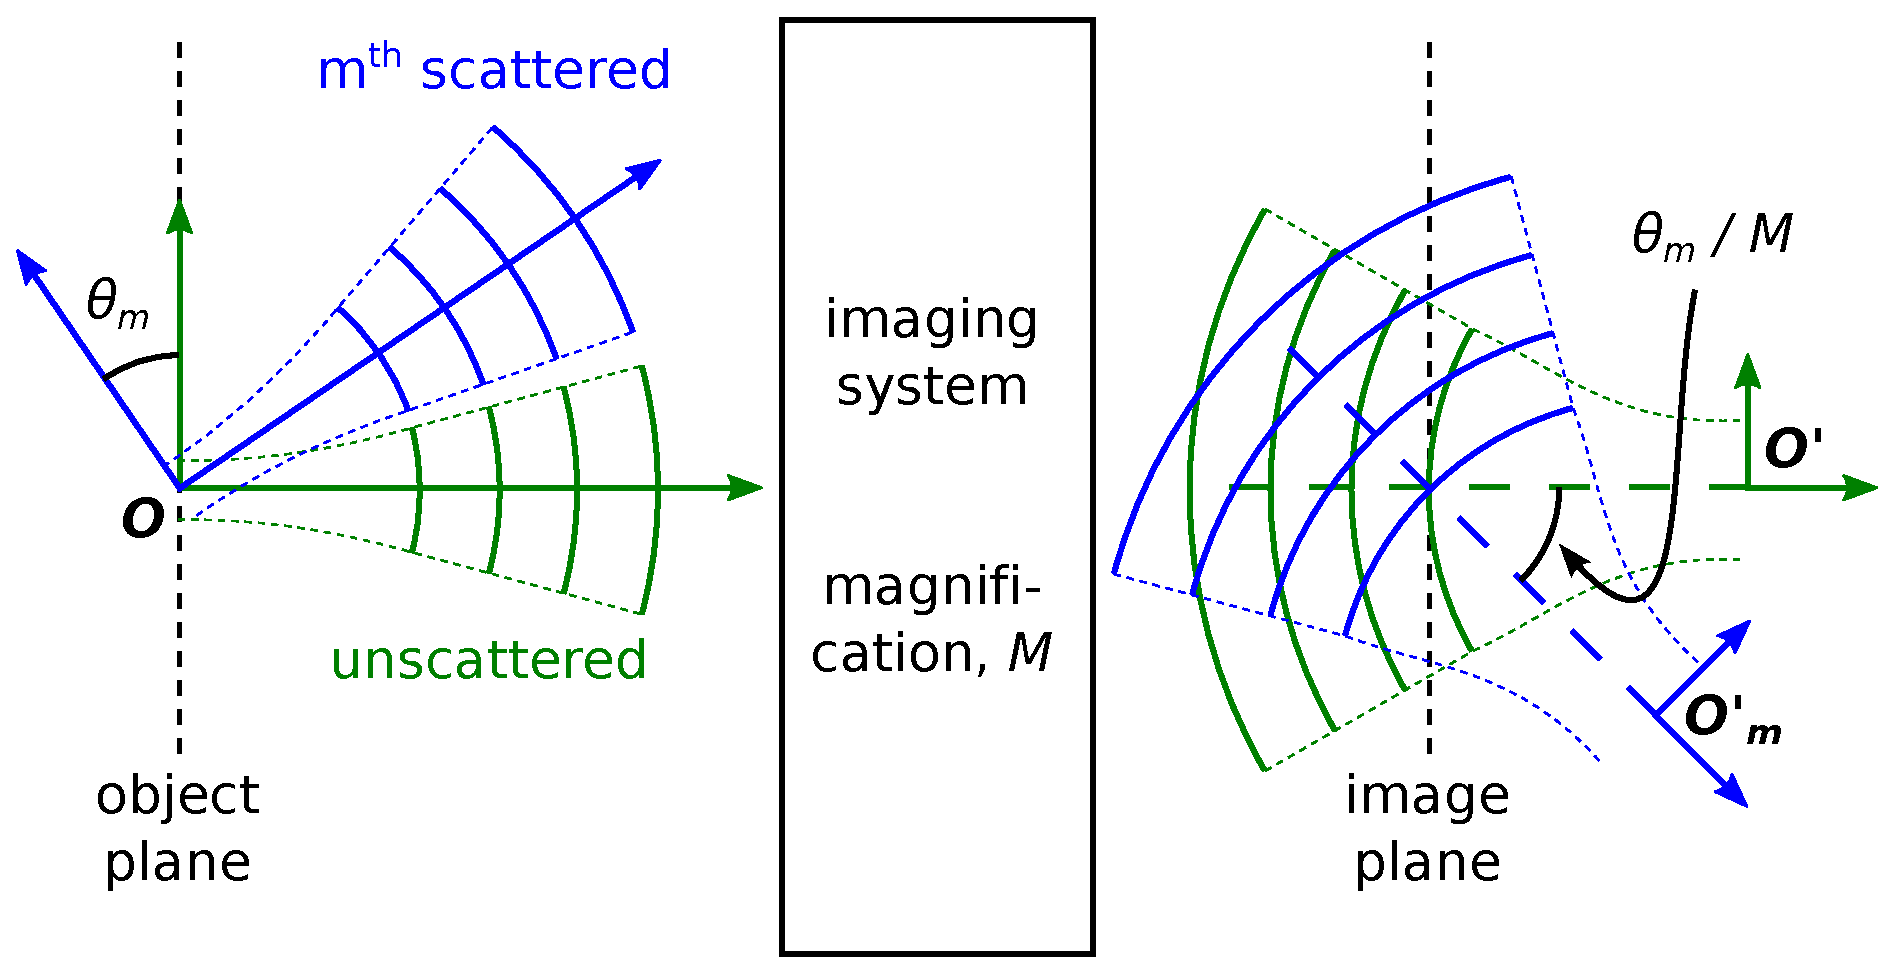
\includegraphics[width = \textwidth]{%
    Chapters/InterferometricMethods/figs/imaging_geometry.eps}
  \caption[Imaging geometry]{%
    Beam geometries in an imaging system with magnification $M$.
    Beam scattering occurs in the object plane at the probe beam's waist.
    Thus, the $m$\ts{th} scattered beam
    shares the origin $\vect{O}_{\object}$ with the unscattered beam but
    is angularly separated by $\theta_m$.
    The imaging system redirects all beams emanating from $\vect{O}_{\object}$
    to intersect at angle $\theta_m / M$ in the image plane.
    In general, the image plane does \emph{not} sit at a beam waist
    such that the post-imaging-system beam waists
    of the scattered and unscattered beams do not coincide,
    i.e.\ $\vect{O}_{\image} \neq \vect{O}_{m,\image}$.}
\label{fig:InterferometricMethods:imaging_geometry}
\end{figure}


\subsection{Gaussian beam transformation in an imaging system}
\label{sec:InterferometricMethods:imaging:Gaussian_beam_transformation}
In addition to manipulating the ray-like trajectory
of a Gaussian beam's optical axis,
an imaging system also alters
other important properties of an incident Gaussian beam.
A Gaussian beam is fully characterized by
its in-medium wavelength $\lambda_0 / N$,
its width $w(z_j)$, and
its radius of curvature $R(z_j)$
at a single location $z_j$.
These parameters can be conveniently combined
to define the so-called complex beam parameter $q$
\cite[Sec.~17.1]{siegman_lasers}
\begin{equation}
  \frac{1}{q}
  \equiv
  \frac{1}{R}
  -
  i \left( \frac{\lambda_0}{N \pi w^2} \right).
  \label{eq:InterferometricMethods:complex_beam_parameter_inverse}
\end{equation}
Referencing the Gaussian-beam width
(\ref{eq:InterferometricMethods:Gaussian_beam_width}) and
the Gaussian-beam radius of curvature
(\ref{eq:InterferometricMethods:Gaussian_beam_radius_of_curvature}),
the complex beam parameter can be rewritten as
\begin{equation}
  q = z + i z_R,
  \label{eq:InterferometricMethods:complex_beam_parameter}
\end{equation}
where $z$ is the axial distance from the beam waist.
The Gaussian beam can then be propagated from point $j$ to point $j + 1$ via
\begin{equation}
  q_{j+1}
  =
  \frac{A q_j + B}{C q_j + D},
  \label{eq:InterferometricMethods:complex_beam_parameter_propagation}
\end{equation}
where, amazingly, $A$, $B$, $C$, and $D$
are equal to the corresponding values
of the $ABCD$ ray matrix from geometric optics
\cite[Sec.~20.2]{siegman_lasers} \cite{tovar_generalized_beam_matrices_IV}.
The beam's transverse and angular displacements
relative to the lab-frame optical axis
are similarly governed by the so-called ``$S$-parameter transformation''
\cite{tovar_generalized_beam_matrices_IV}.
It is important to note that the complex beam parameter and its evolution
are \emph{independent} of the beam's transverse and angular displacements
from the lab-frame optical axis
(assuming such displacements do not violate the paraxial limit, of course);
that is, a scattered beam's width and radius of curvature
evolve identically to those of the unscattered beam.

The properties of the image-plane beams are easily determined.
Using the ray matrix of an imaging system from
(\ref{eq:InterferometricMethods:ABCD_imaging}),
the image-plane complex beam parameter $q_{\image}$ is given as
\begin{equation}
  q_{\image}
  =
  \frac{M q_{\object}}{C q_{\object} + (1 / M)},
  \label{eq:InterferometricMethods:complex_beam_parameter_image_plane}
\end{equation}
where $q_{\object}$ is the object-plane complex beam parameter,
and $M$ and $C$ are both real.
Note that the post-imaging-system beam waists
do \emph{not} necessarily sit at the image plane,
in which case the beams' native coordinate systems
are necessarily \emph{displaced} from each other
(i.e.\ $\vect{O}_{\image} \neq \vect{O}_{m,\image}$,
as indicated in Fig.~\ref{fig:InterferometricMethods:imaging_geometry}).
Examining the image-plane complex beam parameter
(\ref{eq:InterferometricMethods:complex_beam_parameter_image_plane})
it is easy to see that the beam waists will not sit at the image plane
when $C q_{\object} \gg 1 / M$ such that
$z_{\image} = \text{Re}(q_{\image}) \approx M / C \neq 0$.

As the native coordinate systems of
the unscattered beam and the $m$\ts{th} scattered beam
do not align in the image plane,
it will be convenient to determine the relevant coordinate transformation.
The transformation is derived for the most general case
in which the beam waists do not sit at the image plane
(i.e.\ $\vect{O}_{\image} \neq \vect{O}_{m,\image}$,
as indicated in Fig.~\ref{fig:InterferometricMethods:imaging_geometry}).
The coordinate transformation is simply a series of translations and rotations
\begin{equation}
  \vect{r}_{m, \image}
  =
  \left[ \vect{R}(\theta_m / M) \right]
  \left[ \vect{r}_{\image} - z_{\image} \hat{\vect{z}} \right]
  +
  z_{\image} \hat{\vect{z}},
\end{equation}
where $\vect{R}(\theta)$ is the rotation matrix given by
(\ref{eq:InterferometricMethods:rotation_matrix}).
Explicitly,
\begin{equation}
  \begin{pmatrix}
    x_{m, \image}
    \\
    y_{m, \image}
    \\
    z_{m, \image}
  \end{pmatrix}
  =
  \begin{pmatrix}
    x_{\image} \cos\left( \frac{\theta_m}{M} \right)
    \\
    y_{\image}
    \\
    z_{\image} + x_{\image} \sin\left( \frac{\theta_m}{M} \right)
  \end{pmatrix}
  \approx
  \begin{pmatrix}
    x_{\image}
    \\
    y_{\image}
    \\
    z_{\image} + x_{\image} \left( \frac{\theta_m}{M} \right)
  \end{pmatrix},
  \label{eq:InterferometricMethods:coordinate_transformation_imaging_plane}
\end{equation}
where the approximation is valid to first order in $\theta_m / M$.


\subsection{The imaged field}
Now, without further ado,
let $\image$ image the object plane $S_{\object}$
such that the diffracted field
(\ref{eq:InterferometricMethods:phase_modulated_Gaussian_beam_diffraction_Fourier_filtered})
is imaged as
\begin{align}
  E(\vect{r}_{\image}, t)
  &=
  \image[ E(\vect{r}_{\object}, t) ]
  \notag \\
  &\begin{aligned}
    =
    e^{i \bar{\phi}}
    \sum_{m = -1}^{1}
    \biggl\{%
      &i^m \left[ J_m(\tilde{\phi}_0) \right]
      \\
      &\times
      \image[E_T(\vect{r}_{m, \object})]
      e^{-i (\omega_0 + m \omega) t}
    \biggr\},
  \end{aligned}
  \label{eq:InterferometricMethods:imaged_total_field_v1}
\end{align}
where the linearity of $\image$ has been invoked
to bring the operator within the summation.
Referencing the definition of $E_T(\vect{r}_{m})$
(\ref{eq:InterferometricMethods:mth_diffracted_beam_kx_filtered_compact}),
it readily follows that
\begin{align}
  \image[E_T(\vect{r}_{m, \object})]
  &=
  \mathcal{I}[%
    E_G(0, y_{m, \object}, z_{m, \object})
    \cdot
    \mathcal{E}(\vect{r}_{m, \object}, k)
  ]
  \notag \\
  &=
  E_G(0, y_{m, \image}, z_{m, \image})
  \cdot
  \mathcal{E}(\vect{r}_{m, \image}, k_{\image})
  \notag \\
  &\approx
  E_G(0, y_{\image}, z_{\image})
  e^{i m k_{\image} x_{\image}}
  \cdot
  \mathcal{E}(\vect{r}_{m, \image}, k_{\image}),
\end{align}
where the last step naturally follows from
the image-plane coordinate transformation
(\ref{eq:InterferometricMethods:coordinate_transformation_imaging_plane})
and the following approximations:
$w(z_{m, \image}) \approx w(z_{\image})$,
$R(z_{m, \image}) \approx R(z_{\image})$, and
$\psi(z_{m, \image}) \approx \psi(z_{\image})$.
Thus, the imaged field
(\ref{eq:InterferometricMethods:imaged_total_field_v1}) becomes
\begin{equation}
  \begin{aligned}
    E(\vect{r}_{\image}, t)
    &=
    E_G(0, y_{\image}, z_{\image}, t)
    e^{i \bar{\phi}}
    \\
    &\quad \times
    \sum_{m = -1}^{1}
    i^m \left[ J_m(\tilde{\phi}_0) \right]
    \mathcal{E}(\vect{r}_{m, \image}, k_{\image})
    e^{i m \nu},
  \end{aligned}
  \label{eq:InterferometricMethods:imaged_total_field}
\end{equation}
where
\begin{equation}
  \nu
  =
  k_{\image} x_{\image} - \omega t
  \label{eq:InterferometricMethods:image_plane_nu}
\end{equation}
and
$E_G(0, y_{\image}, z_{\image}, t)
=
E_G(0, y_{\image}, z_{\image}) e^{-i \omega_0 t}$.


\subsection{The weak-coupling limit}
\label{sec:InterferometricMethods:imaging:weak_coupling_limit}
Typically, the phase-fluctuation amplitude
is very small ($\tilde{\phi}_0 \ll 1$), and
the Bessel function's small-argument limiting form \cite{abramowitz_and_stegun}
can be used
\begin{equation}
  \lim_{z \rightarrow 0} J_m(z)
  \sim
  \begin{cases}
    \frac{1}{\Gamma(m + 1)} \left( \frac{z}{2} \right)^m
    , \qquad
    &m = 0, 1, 2, 3, \cdots,
    \\
    \frac{1}{\Gamma(|m| + 1)} \left( \frac{-z}{2} \right)^{|m|}
    , \qquad
    &m = -1, -2, -3, \cdots.
  \end{cases}
\end{equation}
Here, $\Gamma$ is the gamma function, and
$\Gamma(m + 1) = m!$ for positive integer $m$.
Introducing the notational shorthand
$\mathcal{E}_m \equiv \mathcal{E}(\vect{r}_{m, \image}, k_{\image})$,
the imaged field to first order in $\tilde{\phi}_0$
(\ref{eq:InterferometricMethods:imaged_total_field}) becomes
\begin{equation}
  \begin{aligned}
  E(\vect{r}_{\image}, t)
  &\approx
  E_G(0, y_{\image}, z_{\image}, t)
  e^{i \bar{\phi}}
  \\
  &\quad\times
  \biggl\{%
    \mathcal{E}_{0}
    +
    i \frac{\tilde{\phi}_0}{2}
    \left[
      \mathcal{E}_{1} e^{i \nu}
      +
      \mathcal{E}_{-1} e^{-i \nu}
    \right]
  \biggr\}.
  \end{aligned}
  \label{eq:InterferometricMethods:imaged_total_field_weak_coupling_Fourier_filtered}
\end{equation}
When there is no wavenumber-dependent manipulation of the scattered beams
(i.e.\ $T(k_x) = 1$), the imaged field
(\ref{eq:InterferometricMethods:imaged_total_field_weak_coupling_Fourier_filtered})
readily reduces to
\begin{equation}
  E(\vect{r}_{\image}, t)
  \approx
  E_G(\vect{r}_{\image}, t)
  e^{i \bar{\phi}}
  \left[%
    1
    +
    i \tilde{\phi}_0 \cos\nu
  \right],
  \label{eq:InterferometricMethods:imaged_total_field_weak_coupling}
\end{equation}
which follows naturally from the image-plane coordinate transformation
(\ref{eq:InterferometricMethods:coordinate_transformation_imaging_plane})
and the following approximations:
$w(z_{m, \image}) \approx w(z_{\image})$ and
$R(z_{m, \image}) \approx R(z_{\image})$.


\subsection{The need for a reference beam}
\label{sec:InterferometricMethods:imaging:need_for_reference_beam}
Assume that there is
no wavenumber-dependent manipulation of the diffracted field
such that
(\ref{eq:InterferometricMethods:imaged_total_field_weak_coupling})
yields the imaged field.
Now, most detectors of interest are square-law detectors
in that they produce a response proportional to
the square (i.e.\ intensity) of the impinging field.
If such a detector is placed at the image plane,
the local intensity is
\begin{align}
  I(\vect{r}_{\image}, t)
  &\equiv
  \frac{c \varepsilon_0}{2} |E(\vect{r}_{\image}, t)|^2
  \notag \\
  &=
  I_G(\vect{r}_{\image})
  [1 + \mathcal{O}(\tilde{\phi}_0)^2],
  \label{eq:InterferometricMethods:imaged_field_intensity}
\end{align}
where
\begin{equation}
  I_G(\vect{r}_{\image})
  =
  \frac{c \varepsilon_0 |E_G(\vect{r}_{\image})|^2}{2}
  \label{eq:InterferometricMethods:Gaussian_beam_intensity}
\end{equation}
is the intensity profile (averaged over an optical cycle)
of the unscattered Gaussian beam.
Thus, for the typical $\tilde{\phi}_0 \ll 1$ limit,
the measured response will be very weak
if the detector is only exposed to the imaged radiation.
Physically, this is attributable to the $m = \pm 1$ beams
being $\pi / 2$ out of phase with the unscattered $m = 0$ beam.
As will be shown in Sections
\ref{sec:InterferometricMethods:interferometry} and
\ref{sec:InterferometricMethods:pci},
the system response can be substantially improved
by interfering the scattered beams with a reference beam.
The generation of such a reference beam, then, is the trait
that differentiates a given interferometric method from another.


\section{External reference-beam interferometry}
\label{sec:InterferometricMethods:interferometry}
In external reference-beam interferometry,
there is no wavenumber-dependent manipulation of the diffracted field
such that
(\ref{eq:InterferometricMethods:imaged_total_field_weak_coupling})
yields the imaged field.
Thus, the probe radiation in the image plane is given as
\begin{equation}
  E_P(\vect{r}_{\image}, t)
  \approx
  E_G(\vect{r}_{\image}, t)
  e^{i \bar{\phi}}
  \left[%
    1
    +
    i \tilde{\phi}_0 \cos\nu
  \right].
\end{equation}
Now, assume that the imaged probe radiation
is interfered with a reference beam of known phase $\phi_R$
\begin{equation}
  E_R(\vect{r}_{\image}, t) = E_G(\vect{r}_{\image}, t) e^{i \phi_R}.
  \label{eq:InterferometricMethods:external_reference_beam_arbitrary}
\end{equation}
The total field impinging on the detector is then
\begin{equation}
  E(\vect{r}_{\image}, t)
  =
  E_G(\vect{r}_{\image}, t)
  \left[%
    e^{i \phi_R}
    +
    e^{i \bar{\phi}}
    \left(%
      1
      +
      i \tilde{\phi}_0 \cos\nu
    \right)
  \right],
\end{equation}
and, to first order in $\tilde{\phi}_0$, the corresponding intensity is
\begin{equation}
  I(\vect{r}_{\image}, t)
  =
  2 I_G(\vect{r}_{\image})
  \left[%
    1
    +
    \cos(\phi_R - \bar{\phi})
    +
    \tilde{\phi}_0 \sin(\phi_R - \bar{\phi}) \cos\nu
  \right],
  \label{eq:InterferometricMethods:interferometer_intensity_arbitrary_reference}
\end{equation}
where $I_G(\vect{r}_{\image})$ is
the intensity profile of the unscattered Gaussian beam on the detector
as defined in (\ref{eq:InterferometricMethods:Gaussian_beam_intensity}).
Reference-beam generation prescribes $\phi_R$ and
consequently dictates the method of interferometric detection.


\subsection{Homodyne detection}
\label{sec:InterferometricMethods:interferometry:homodyne}
\begin{figure}
  \centering
  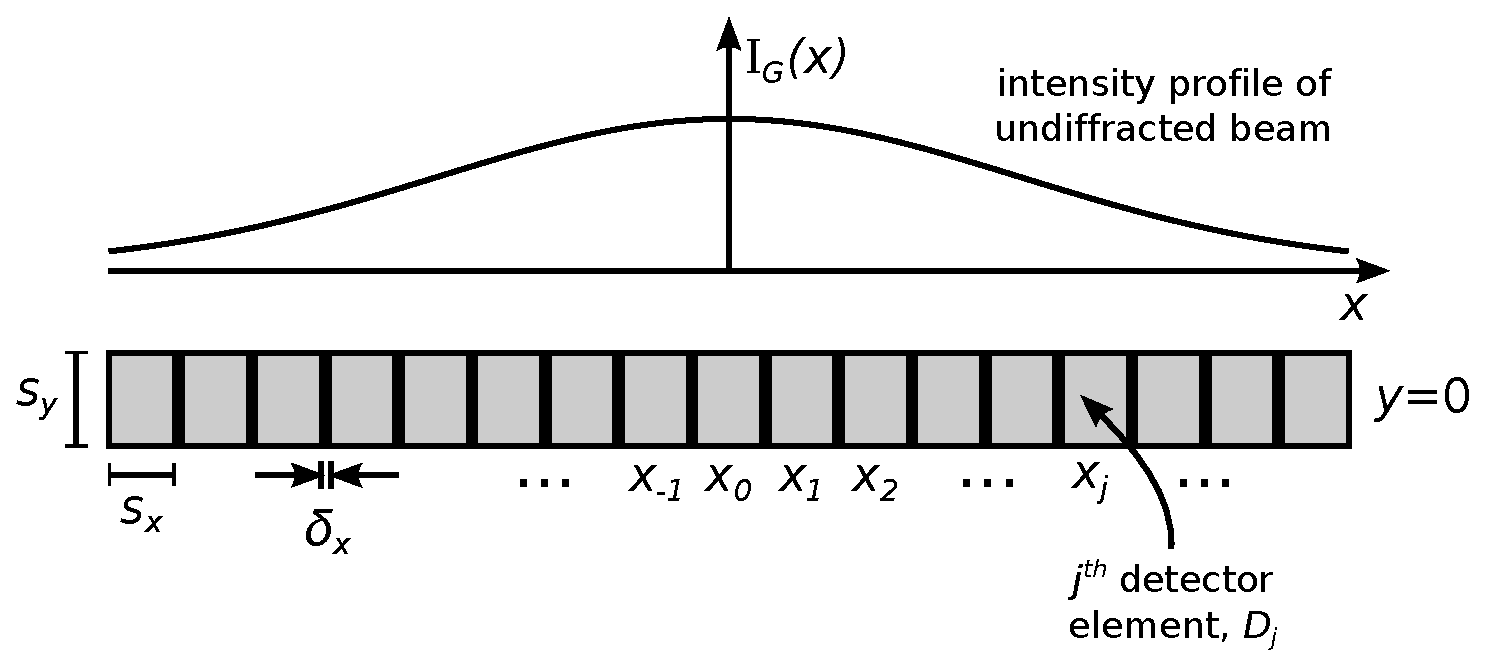
\includegraphics[width = \textwidth]{%
    Chapters/InterferometricMethods/figs/detector_array.eps}
  \caption[Finite sampling-volume effects in a detector array]{%
    The probe radiation and the reference beam
    are interfered on a detector array.
    The array consists of numerous detector elements,
    each of size $s_x \times s_y$ and with interelement spacing $\delta_x$.
    The unscattered beam is centered on $x_0 = 0$ and $y = 0$, and
    its intensity profile varies only weakly over any given element.
    The finite size of each detector element tends to attenuate
    short wavelength components of the incident optical signal.
  }
  \label{fig:InterferometricMethods:detector_array}
\end{figure}

Homodyne detection results from using
a reference phase that is constant (or nearly constant) in time
such that the resulting intensity is
\begin{equation}
  \begin{aligned}
    I_{\text{hom}}(\vect{r}_{\image}, t)
    =
    2 I_G(\vect{r}_{\image})
    \bigl[%
      1
      &+
      \cos(\phi_R - \bar{\phi})
      \\
      &+
      \tilde{\phi}_0
      \sin(\phi_R - \bar{\phi}) \cos\nu
    \bigr].
  \end{aligned}
  \label{eq:InterferometricMethods:homodyne_intensity}
\end{equation}
Finite sampling-volume effects~\cite{bravenec_rsi95} dictate
the homodyne interferometer's wavenumber response~\cite{davis_rsi16}.
Assume that the probe radiation and the reference beam
are interfered on a detector array,
as shown in Fig.~\ref{fig:InterferometricMethods:detector_array}.
Let the $j$\ts{th} detector element $D_j$ be centered on $x_{\image,j}$
and $y_{\image} = 0$;
the total power $P_{j, \, \text{hom}}$ incident on this element is then
\begin{align}
  P_{j, \, \text{hom}}(t)
  &=
  \int_{D_j} I_{\text{hom}}(\vect{r}_{\image}, t) dA
  \notag \\
  &\begin{aligned}
    \approx
    2 I_G(\vect{r}_{\image,j}) s_y
    &\int_{x_{\image,j} - s_x / 2}^{x_{\image,j} + s_x / 2}
    \biggl[%
      1
      +
      \cos(\phi_R - \bar{\phi})
      \\
      &\qquad+
      \tilde{\phi}_0
      \sin(\phi_R - \bar{\phi}) \cos\nu
    \biggr] dx_{\image},
  \end{aligned}
  \label{eq:InterferometricMethods:homodyne_interferometer_total_power_per_element_integral}
\end{align}
where the weakly varying intensity profile $I_G(\vect{r}_{\image})$
has been approximated as a constant
over the face of the detector element.
As the finite sampling-volume integral
will also be applied in other sections,
it is explicitly evaluated here for later reference
\begin{equation}
  \int_{x_{\image,j} - s_x / 2}^{x_{\image,j} + s_x / 2}
  \cos(\nu + \theta) dx_{\image}
  =
  s_x
  \cdot
  T_{\text{fsv}}(k_{\image})
  \cdot
  \cos(\nu_j + \theta),
  \label{eq:InterferometricMethods:finite_sampling_volume_integral}
\end{equation}
where
\begin{equation}
  T_{\text{fsv}}(k_{\image})
  \equiv
  \sinc\left( \frac{k_{\image}}{k_{\text{fsv},\image}} \right)
  \label{eq:InterferometricMethods:finite_sampling_volume_transfer_function}
\end{equation}
is the finite sampling-volume transfer function,
\begin{equation}
  \sinc(x) = \frac{\sin(\pi x)}{\pi x}
  \label{eq:InterferometricMethods:normalized_sinc}
\end{equation}
is the normalized sinc function,
\begin{equation}
  k_{\text{fsv},\image} = \frac{2 \pi}{s_x}
  \label{eq:InterferometricMethods:finite_sampling_volume_cutoff}
\end{equation}
is the first zero of $T_{\text{fsv}}(k_{\image})$,
\begin{equation}
  \nu_j = k_{\image} x_{\image,j} - \omega t,
  \label{eq:InterferometricMethods:nu_j}
\end{equation}
and $\theta$ is a \emph{constant} with respect to $x_{\image}$.
Thus, the homodyne optical power becomes
\begin{align}
  \begin{aligned}
    P_{j, \, \text{hom}}(t)
    =
    2 I_G(\vect{r}_{\image,j}) A
    &\bigl[%
      1
      +
      \cos(\phi_R - \bar{\phi})
      \\
      &+
      \tilde{\phi}_0
      \sin(\phi_R - \bar{\phi})
      T_{\text{fsv}}(k_{\image})
      \cos\nu_j
    \bigr],
  \end{aligned}
  \label{eq:InterferometricMethods:homodyne_interferometer_total_power_per_element}
\end{align}
where $A = s_x s_y$ is the area of the detector element.

The typical engineering constraint of such a system
is the saturation intensity of the detector elements.
Beyond the linear saturation intensity $I_{\text{sat}}$,
the detector's response ceases to be a linear function
of the incident optical power.
For approximately uniform illumination,
the saturation threshold can be equivalently characterized
by a saturation power $P_{\text{sat}} \equiv I_{\text{sat}} A$.
To make an ``apples-to-apples'' comparison of different interference schemes,
it is useful to examine the ratio of the fluctuating power to $P_{\text{sat}}$.
To proceed, note that the homodyne optical power in
(\ref{eq:InterferometricMethods:homodyne_interferometer_total_power_per_element})
can be separated into equilibrium and fluctuating components as
$P_{j, \, \text{hom}}(t)
=
\bar{P}_{j, \, \text{hom}}
+
\tilde{P}_{j, \, \text{hom}}(t)$, where
\begin{align}
  \bar{P}_{j, \, \text{hom}}(t)
  &=
  2 I_G(\vect{r}_{\image,j}) A
  [1 + \cos(\phi_R - \bar{\phi})],
  \\
  \tilde{P}_{j, \, \text{hom}}(t)
  &=
  2 I_G(\vect{r}_{\image,j}) A
  \tilde{\phi}_0
  \sin(\phi_R - \bar{\phi})
  T_{\text{fsv}}(k_{\image})
  \cos\nu_j.
\end{align}
Then, because $\tilde{\phi}_0 \ll 1$
\begin{equation}
  P_{j, \, \text{hom}}
  \approx
  \bar{P}_{j, \, \text{hom}}
  \leq
  2 I_G(0) A [1 + \cos(\phi_R - \bar{\phi})],
  \notag
\end{equation}
where $I_G(0)$ is the peak intensity of the unscattered Gaussian probe beam.
To obtain optimal performance, select $I_G(0)$ such that
\begin{equation}
  P_{\text{sat}}
  =
  2 I_G(0) A [1 + \cos(\phi_R - \bar{\phi})].
  \notag
\end{equation}
Then
\begin{equation}
  \frac{\tilde{P}_{j, \, \text{hom}}(t)}{P_{\text{sat}}}
  =
  \frac{I_G(\vect{r}_{\image,j})}{I_G(0)}
  \cdot
  T_{\text{hom}}(k_{\image})
  \cdot
  \tilde{\phi}_0 \cos\nu_j,
\end{equation}
where
\begin{equation}
  T_{\text{hom}}(k_{\image})
  \equiv
  \frac{\sin(\phi_R - \bar{\phi})}{1 + \cos(\phi_R - \bar{\phi})}
  \cdot
  T_{\text{fsv}}(k_{\image})
  \label{eq:InterferometricMethods:homodyne_interferometer_wavenumber_transfer_function}
\end{equation}
is the homodyne interferometer's wavenumber transfer function.
That is, the homodyne interferometer
weights the phase-fluctuation images $\tilde{\phi}_0 \cos\nu_j$
by its transfer function $T_{\text{hom}}(k_{\image})$.
The prefactor $I_G(\vect{r}_{\image,j}) / I_G(0)$
can (and should) be accounted for
if the beam profile is known.

Note that $T_{\text{hom}}(k_{\image})$ is a function
of the phase difference $\phi_R - \bar{\phi}$.
The homodyne interferometer operates at its peak sensitivity
when $|T_{\text{hom}}(k_{\image})|$ is maximal,
which occurs when $\phi_R - \bar{\phi} = \pi / 2 + m \pi$ for integer $m$.
For concreteness in the following discussion,
take $\phi_R - \bar{\phi} = \pi / 2$.
Physically, $\phi_R - \bar{\phi} = \pi / 2$
means that the reference beam is
out-of-phase with the unscattered beam but
in-phase with the scattered beams.
Note that interfering the scattered beams with this in-phase reference beam
produces an intensity linear in $\tilde{\phi}_0$;
this should be contrasted with the weak, quadratic intensity variation
of (\ref{eq:InterferometricMethods:imaged_field_intensity})
that occurs in the absence of a reference beam

Practically speaking, however,
it is very difficult to keep $\phi_R - \bar{\phi}$ fixed at $\pi / 2$.
First, a CO$_2$ beam passing through $\sim \SI{1}{\meter}$
of plasma with a density $n_e \sim \SI{e20}{\per\meter\cubed}$
will experience a bulk phase delay $\bar{\phi} \sim \pi$;
thus, for constant $\phi_R$, it will be impossible
to operate the interferometer at its peak sensitivity
($\phi_R - \bar{\phi} \approx \pi / 2$)
as the density evolves across the discharge.
Second, fusion experiments are often characterized
by large, pulsed electromagnets
whose vibrations can change the path lengths of the interferometer's arms.
A path-length change $\delta l$ produces
$\delta(\phi_R - \bar{\phi}) = k_0 \delta l$,
where $k_0$ is the wavenumber of the probe radiation.
For a $\SI{10.6}{\micro\meter}$ CO$_2$ probe beam,
a path-length variation $\sim \SI{2.5}{\micro\meter}$
is sufficient to produce $\delta(\phi_R - \bar{\phi}) \sim \pi / 2$,
pushing the homodyne interferometer from
its configuration of peak sensitivity into one of its nulls.
Even vacuum-pump vibrations can provide such a push!
On small fusion devices,
actively controlled mirrors have been used in an attempt
to account for the evolution of the equilibrium phase and
to cancel vibrational path-length changes,
minimizing excursions from $\phi_R - \bar{\phi} \approx \pi / 2$
\cite{nazikian_rsi87}, but
such an approach has not found application on larger
(and presumably more vibration-prone) fusion experiments.

In addition to its variable sensitivity,
the homodyne interferometer does \emph{not} make an absolute measurement
of the phase fluctuation amplitude $\tilde{\phi}_0$
\cite[Sec.~4.2.2]{hutchinson_diagnostics}.
For example, vibration-induced misalignment or
power fluctuations at the beam source
can alter the intensity $I_G(\vect{r}_{\image,j})$.
As a result, there are three potentially dynamic quantities:
$\{\phi_R - \bar{\phi}, \tilde{\phi}_0, I_G(\vect{r}_{\image,j})\}$, but
there are only two measured quantities:
the equilibrium and fluctuating homodyne powers.
Thus, it is generally impossible to distinguish
whether changes in the amplitude of the fluctuating power
are attributable to real changes in $\tilde{\phi}_0$ or
are simply an artifact of the system alignment or radiation source.


\subsection{Heterodyne detection}
To avoid the above-mentioned challenges of homodyne interferometry,
the reference phase can be linearly ramped in time
as $\phi_R = \Delta \omega_0 t$ such that
the intensity becomes
\begin{equation}
  \begin{aligned}
    I_{\text{het}}(\vect{r}_{\image}, t)
    =
    2 I_G(\vect{r}_{\image})
    \bigl[%
      1
      &+
      \cos(\Delta \omega_0 t - \bar{\phi})
      \\
      &+
      \tilde{\phi}_0
      \sin(\Delta \omega_0 t - \bar{\phi}) \cos\nu
    \bigr].
  \end{aligned}
  \label{eq:InterferometricMethods:heterodyne_intensity}
\end{equation}
This approach is known as heterodyne interferometry,
as the desired baseband phase information is shifted
to an intermediate frequency $\Delta \omega_0$
satisfying $\omega \ll \Delta \omega_0 \ll \omega_0$.
The effect on the frequency-space representation
of the interference signal is sketched in
Fig.~\ref{fig:InterferometricMethods:baseband_vs_intermediate_frequency}.
\graffito{\textcolor{red}{This will be discussed more in Ch.~3}}
Practically, the $\phi_R$ ramp is accomplished by modestly Doppler shifting
the reference beam relative to the plasma beam.

\begin{figure}
  \centering
  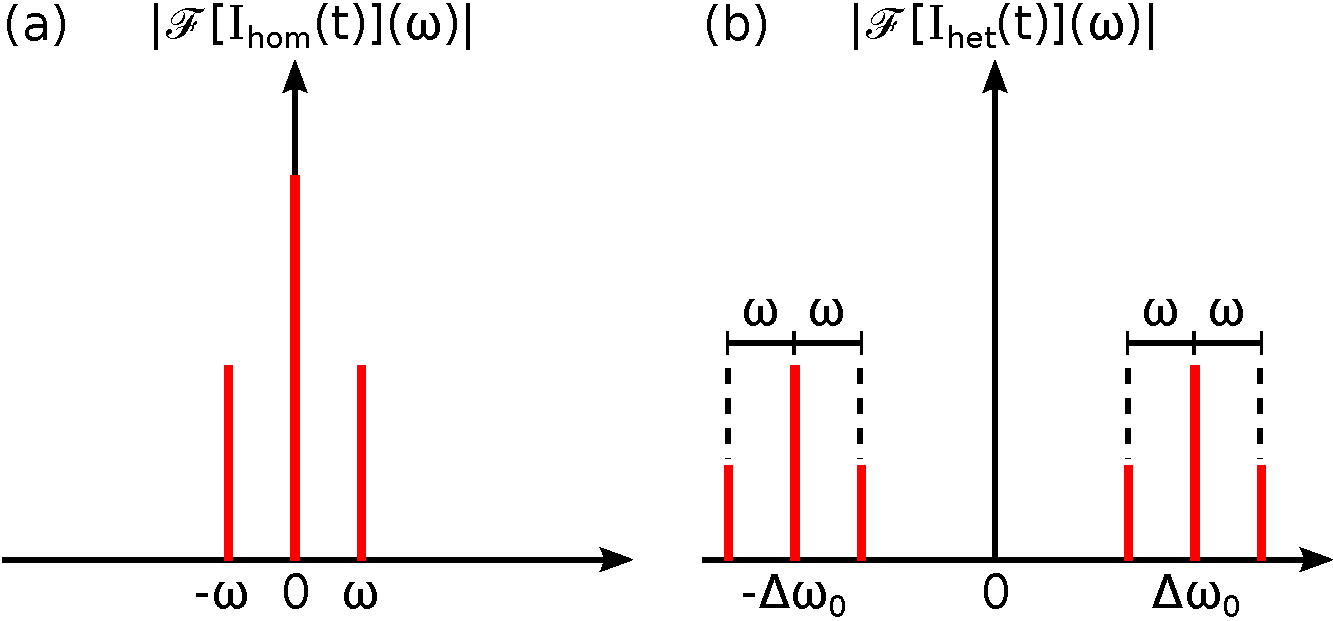
\includegraphics[width = \textwidth]{%
    Chapters/InterferometricMethods/figs/baseband_vs_intermediate_frequency.pdf}
  \caption[Schematic of homodyne vs.\ heterodyne signals in frequency space]{%
    Schematic of (a) homodyne vs.\ (b) heterodyne signals in frequency space.
    A homodyne signal is predominantly DC, and
    a sinusoidal fluctuation with angular frequency $\omega$
    produces sidebands at $\pm \omega$.
    In contrast, the power in a heterodyne signal is shifted
    to the intermediate frequencies $\pm \Delta \omega_0$, and
    a sinusoidal fluctuation with angular frequency $\omega$
    produces sidebands at $\Delta \omega_0 \pm \omega$ and
    $-\Delta \omega_0 \pm \omega$.}
  \label{fig:InterferometricMethods:baseband_vs_intermediate_frequency}
\end{figure}

As is the case for homodyne detection,
finite sampling-volume effects~\cite{bravenec_rsi95} dictate
the heterodyne interferometer's wavenumber response~\cite{davis_rsi16}.
The following discussion closely parallels that
of the homodyne interferometer in
Section~\ref{sec:InterferometricMethods:interferometry:homodyne}, and
readers are encouraged to review that section if needed and
to compare and contrast homodyne and heterodyne detection.
Assume that the probe radiation and the reference beam
are interfered on a detector array,
as shown in Fig.~\ref{fig:InterferometricMethods:detector_array}.
Let the $j$\ts{th} detector element $D_j$ be centered on $x_j$ and $y = 0$;
the total power $P_{j, \, \text{het}}$ incident on this element is then
\begin{align}
  P_{j, \, \text{het}}(t)
  &=
  \int_{D_j} I_{\text{het}}(\vect{r}_{\image}, t) dA
  \notag \\
  &\begin{aligned}
    \approx
    2 I_G(\vect{r}_{\image,j}) s_y
    &\int_{x_{\image,j} - s_x / 2}^{x_{\image,j} + s_x / 2}
    \biggl[%
      1
      +
      \cos(\Delta \omega_0 t - \bar{\phi})
      \\
      &\qquad+
      \tilde{\phi}_0
      \sin(\Delta \omega_0 t - \bar{\phi}) \cos\nu
    \biggr] dx
  \end{aligned}
  \notag \\
  &\begin{aligned}
    &=
    2 I_G(\vect{r}_{\image,j}) A
    \biggl[%
      1
      +
      \cos(\Delta \omega_0 t - \bar{\phi})
      \\
      &\qquad+
      \tilde{\phi}_0
      \sin(\Delta \omega_0 t - \bar{\phi})
      T_{\text{fsv}}(k_{\image})
      \cos\nu_j
    \biggr],
  \end{aligned}
  \label{eq:InterferometricMethods:heterodyne_interferometer_total_power_per_element}
\end{align}
where the weakly varying intensity profile $I_G(\vect{r}_{\image})$
has been approximated as a constant
over the face of the detector element, and
the finite sampling-volume integral in
(\ref{eq:InterferometricMethods:finite_sampling_volume_integral})
has been referenced.
Note that the dominant Fourier components of $P_{j, \, \text{het}}$
sit at the intermediate frequency $\pm \Delta \omega_0$ but that
the phase-fluctuation term $\sin(\Delta \omega_0 t - \bar{\phi}) \cos\nu_j$
produces sidebands at $\pm (\Delta \omega_0 \pm \omega)$.

The heterodyne interference signal must be demodulated
in order to retrieve the baseband phase-fluctuation information.
\graffito{\textcolor{red}{More on demodulation hardware in Ch.~3}}
Practically speaking, dedicated analog or digital electronics
are used to demodulate the heterodyne signal;
however, for the pedagogical purposes of this section,
it is sufficient to consider the ``equivalent optical powers''
corresponding to the demodulated signals.
The so-called in-phase ($I$) and quadrature ($Q$) signals
are obtained by mixing $P_{j, \, \text{het}}$ with
$\cos( \Delta \omega_0 t)$ and $\sin( \Delta \omega_0 t)$, respectively, and
low-pass filtering the resulting signals;
here, low-pass filtering is implemented
by averaging over a cycle of the intermediate frequency.
Thus, the equivalent $I$ and $Q$ optical powers are defined as
\begin{align}
  P_{j, I}(t)
  &\equiv
  \langle
    \cos (\Delta \omega_0 t) \cdot P_{j, \, \text{het}}(t)
  \rangle_{\Delta \omega_0},
  \\
  P_{j, Q}(t)
  &\equiv
  \langle
    \sin (\Delta \omega_0 t) \cdot P_{j, \, \text{het}}(t)
  \rangle_{\Delta \omega_0},
\end{align}
where $\langle q \rangle_{\Delta \omega_0}$ denotes
the average of quantity $q$ over an intermediate-frequency cycle as
\begin{equation}
  \langle q \rangle_{\Delta \omega_0}
  \equiv
  \frac{\Delta \omega_0}{2 \pi}
  \int_{0}^{\Delta \omega_0 / 2 \pi}
  q(t) dt.
  \label{eq:InterferometricMethods:intermediate_frequency_cycle_average}
\end{equation}
Note that $P_{j,I}$ and $P_{j,Q}$ can be conveniently combined as
\begin{align}
  P_{j,I} + i \cdot P_{j,Q}
  &=
  \langle
    e^{i \Delta \omega_0 t} \cdot P_{j, \, \text{het}}(t)
  \rangle_{\Delta \omega_0}
  \notag \\
  &=
  I_G(\vect{r}_{\image,j}) A
  e^{i \bar{\phi}}
  \left[%
    1
    +
    i \tilde{\phi}_0
    T_{\text{fsv}}(k_{\image})
    \cos\nu_j
  \right].
  \label{eq:InterferometricMethods:heterodyne_interferometer_I_and_Q_power_per_element}
\end{align}

In contrast to the homodyne interferometer,
the heterodyne interferometer makes an absolute measurement
of the phase-fluctuation amplitude $\tilde{\phi}_0$.
To see this, note that $P_{j,I}$ and $P_{j,Q}$
(the real and imaginary components of
(\ref{eq:InterferometricMethods:heterodyne_interferometer_I_and_Q_power_per_element}),
respectively)
can be separated into equilibrium and fluctuating components as
\begin{align}
  \bar{P}_{j,I}(t)
  &=
  I_G(\vect{r}_{\image,j}) A \cos\bar{\phi},
  \\
  \bar{P}_{j,Q}(t)
  &=
  I_G(\vect{r}_{\image,j}) A \sin\bar{\phi},
  \\
  \tilde{P}_{j,I}(t)
  &=
  -I_G(\vect{r}_{\image,j}) A
  \tilde{\phi}_0
  \sin\bar{\phi} \,
  T_{\text{fsv}}(k_{\image})
  \cos\nu_j,
  \\
  \tilde{P}_{j,Q}(t)
  &=
  I_G(\vect{r}_{\image,j}) A
  \tilde{\phi}_0
  \cos\bar{\phi} \,
  T_{\text{fsv}}(k_{\image})
  \cos\nu_j.
\end{align}
As is the case for the homodyne interferometer,
there are three potentially dynamic quantities:
$\{\bar{\phi}, \tilde{\phi}_0, I_G(\vect{r}_{\image,j})\}$;
however, in contrast to the homodyne interferometer,
there are now \emph{four} measured quantities:
$\{\bar{P}_{j,I}, \bar{P}_{j,Q}, \tilde{P}_{j,I}, \tilde{P}_{j,Q}\}$.
Therefore, the number of measured quantities
is sufficient to unambiguously determine
$\{\bar{\phi}, \tilde{\phi}_0, I_G(\vect{r}_{\image,j})\}$
in absolute units.

Finally, it is useful to characterize
the heterodyne interferometer's performance
relative to the saturation limits of a given detector.
Because $\tilde{\phi}_0 \ll 1$,
the heterodyne power incident on the $j$\ts{th} detector element
(\ref{eq:InterferometricMethods:heterodyne_interferometer_total_power_per_element})
can be approximated as
\begin{align}
  P_{j, \, \text{het}}
  &\approx
  2 I_G(\vect{r}_{\image,j}) A [1 + \cos(\Delta \omega_0 t - \bar{\phi})]
  \notag \\
  &\leq
  4 I_G(0) A,
  \notag
\end{align}
where $I_G(0)$ is the peak intensity of the unscattered Gaussian probe beam.
To obtain optimal performance, select $I_G(0)$ such that
\begin{equation}
  P_{\text{sat}}
  =
  4 I_G(0) A.
  \notag
\end{equation}
Further, define the total fluctuating power
in the demodulated signals to be
\begin{align}
  \tilde{P}_{j, IQ}(t)
  &\equiv
  \left\{%
    [\tilde{P}_{j,I}(t)]^2
    +
    [\tilde{P}_{j,Q}(t)]^2
  \right\}^{1/2}
  \notag \\
  &=
  I_G(\vect{r}_{\image,j}) A
  \tilde{\phi}_0
  T_{\text{fsv}}(k_{\image})
  \cos\nu_j
\end{align}
such that
\begin{equation}
  \frac{\tilde{P}_{j, IQ}(t)}{P_{\text{sat}}}
  =
  \frac{I_G(\vect{r}_{\image,j})}{I_G(0)}
  \cdot
  T_{\text{het}}(k_{\image})
  \cdot
  \tilde{\phi}_0
  \cos\nu_j,
\end{equation}
where
\begin{equation}
  T_{\text{het}}(k_{\image})
  \equiv
  \frac{T_{\text{fsv}}(k_{\image})}{4}
  \label{eq:InterferometricMethods:heterodyne_interferometer_wavenumber_transfer_function}
\end{equation}
is the heterodyne interferometer's wavenumber transfer function.
That is, the heterodyne interferometer
weights the phase-fluctuation images $\tilde{\phi}_0 \cos\nu_j$
by its transfer function $T_{\text{het}}(k_{\image})$.
The prefactor $I_G(\vect{r}_{\image,j}) / I_G(0)$
can (and should) be accounted for
if the beam profile is known.

In contrast to the homodyne interferometer,
the heterodyne interferometer's wavenumber transfer function
is \emph{not} a function of $\phi_R - \bar{\phi}$.
Thus, the heterodyne interferometer always operates at its peak sensitivity,
regardless of the bulk plasma phase or path-length vibrations.
Robust sensitivity comes at a cost, however.
Note that
\begin{equation}
  \frac{T_{\text{het}}(k_{\image})}{T_{\text{hom}}(k_{\image})}
  =
  \frac{1}{4}
  \quad
  \text{for homodyne operation at $\phi_R - \bar{\phi} = \pi / 2$.}
  \notag
\end{equation}
Thus, for a given detector,
a heterodyne interferometer will be four times \emph{less} sensitive
than a homodyne interferometer operated in its optimal configuration
($\phi_R - \bar{\phi} = \pi / 2$).
This factor of four has two physical origins.
First, the detector of a homodyne interferometer
with a fixed $\phi_R - \bar{\phi} = \pi / 2$
only sees small fluctuations about a DC offset, while
the detector of a heterodyne interferometer
sees the full sinusoidal waveform of the intermediate frequency;
to ensure the detector is always within its saturation limits,
the heterodyne interferometer must necessarily be operated with
a mean intensity at the detector
that is a factor of two lower than that for the homodyne interferometer.
Second, the mixing process
that is used to demodulate the heterodyne interference signal
results in a loss of half of the signal power.


\section{Phase contrast imaging (PCI)}
\label{sec:InterferometricMethods:pci}
As discussed in
Section~\ref{sec:InterferometricMethods:imaging:need_for_reference_beam},
imaging the probe radiation on a square-law detector
produces a very weak response
because the unscattered and scattered beams
are $\pi / 2$ out of phase with each other.
To produce a measurable response, a traditional interferometer
interferes the imaged radiation with an external reference beam.
If the phase of the unscattered beam could be manipulated, though,
the external reference beam would no longer be needed.
This is the approach employed in phase contrast imaging (PCI).
A typical PCI system is shown schematically in
Fig.~\ref{fig:InterferometricMethods:pci_schematic}.

\begin{figure}
  \centering
  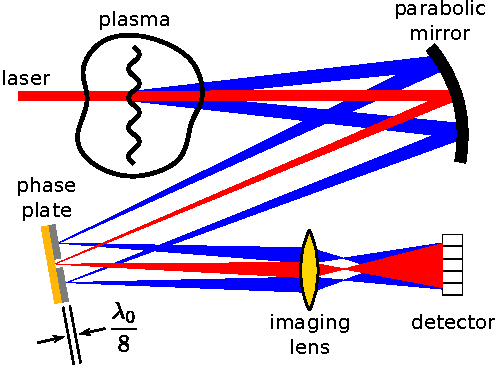
\includegraphics[width = 0.75 \textwidth]{%
    Chapters/InterferometricMethods/figs/pci_schematic.pdf}
  \caption[Schematic overview of a typical PCI system]{%
    Schematic overview of a typical PCI system.
    A plasma-density fluctuation weakly scatters an incident probe beam, and
    an off-axis parabolic mirror focuses the scattered and unscattered beams.
    An optical element known as a phase plate
    is placed at the focal plane of the parabolic mirror.
    The phase plate has a narrow groove of depth $\lambda_0 / 8$
    that imparts phase delay $\pi / 2$ to the unscattered beam,
    effectively converting the unscattered beam
    into an ``internal'' reference beam
    against which the scattered beams can be interfered.
    A lens, whose object plane sits at the plasma midplane,
    is then used to image the resulting radiation onto a detector array.}
  \label{fig:InterferometricMethods:pci_schematic}
\end{figure}


\subsection{Reference-beam generation with a phase plate}
PCI uses an optical element known as a \emph{phase plate}
to delay the unscattered beam by $\pi / 2$
relative to the scattered beams.
The phase plate is typically a reflective optical element
with a groove that is precisely fabricated
to have a depth of $\lambda_0 / 8$;
the unscattered beam reflects off of this groove, and
the corresponding $\lambda_0 / 4$-increase in path length
phase delays the unscattered beam by $\pi / 2$
relative to the scattered beams,
which reflect off of the non-grooved portions
(i.e.\ the ``face'') of the phase plate.
To boost the relative size of the fluctuating signal,
the phase groove typically reflects only a fraction $\eta < 1$
of the incident unscattered beam power, while
the phase-plate face reflects all of the scattered beam power.
Thus, by the action of the phase plate,
$1 \rightarrow i \sqrt{\eta}$ in the imaged electric field
(\ref{eq:InterferometricMethods:imaged_total_field_weak_coupling})
such that
\begin{equation}
  E_{\text{PCI}}(\vect{r}_{\image}, t)
  =
  i E_G(\vect{r}_{\image}, t) e^{i \bar{\phi}}
  \left[%
    \sqrt{\eta} + \tilde{\phi}_0 \cos\nu
  \right],
  \label{eq:InterferometricMethods:pci_imaged_field}
\end{equation}
and the corresponding intensity, to first order in $\tilde{\phi}_0$, is
\begin{equation}
  I_{\text{PCI}}(\vect{r}_{\image}, t)
  =
  I_G(\vect{r}_{\image})
  \left[%
    \eta
    +
    2 \sqrt{\eta} \tilde{\phi}_0 \cos\nu
  \right].
  \label{eq:InterferometricMethods:pci_intensity}
\end{equation}
Here, $E_G(\vect{r}_{\image})$ and $I_G(\vect{r}_{\image})$
are the field and intensity profiles
of the unscattered Gaussian beam on the detector
in the \emph{absence} of the phase plate,
with $I_G(\vect{r}_{\image})$ being explicitly defined in
(\ref{eq:InterferometricMethods:Gaussian_beam_intensity}).
Equation
(\ref{eq:InterferometricMethods:pci_intensity})
should be contrasted with
(\ref{eq:InterferometricMethods:imaged_field_intensity}),
which gives the image-plane intensity
in the absence of the phase plate.
Thus, the phase plate converts the unscattered probe beam
into an effective reference beam for the scattered beams.


\subsection{Focal-plane separation of scattered beams}
Implicit in the use of the phase plate
is that the scattered and unscattered beams
are well-separated in space
such that the phase groove only affects the unscattered beam.
The 1\ts{st}-order scattered beams are angularly separated
from the unscattered beam by $\theta = k / k_0$, and,
in the far field ($z \gg z_R$),
the center of the scattered beam will fall outside of
the unscattered beam's 1/e $E$ radius if
\begin{equation}
  |k| \geq \frac{2}{w_0}.
  \label{eq:InterferometricMethods:kmin_for_far_field_beam_separation}
\end{equation}
However, CO$_2$ laser beams used to probe tokamak plasmas often have
$z_R \gg \SI{10}{\meter}$, so
the beam's far field is not easily accessible in typical lab settings.
Fortunately, the far-field diffraction pattern
can be equivalently accessed in the focal plane
of a focusing optic~\cite[Ch.~8]{born_and_wolf}.

The focal-plane location, beam size, and beam separation
can be easily determined.
Let the Gaussian probe beam have
an in-vessel 1/e $E$ waist radius of $w_0$,
and place a focusing optic of focal length $f$
a distance $s$ downstream from the in-vessel beam waist.
Then, the waist of the focused beam
will be located a distance $s'$ downstream of the focusing optic
and will have 1/e $E$ radius $w_0'$ given as
\begin{align}
  s' &= f \left( 1 + \frac{s - f}{z_R} \right),
  \\
  w_0' &= \frac{w_0 |f|}{\left[ (s - f)^2 + z_R^2 \right]^{1/2}},
\end{align}
where $z_R$ is the in-vessel Rayleigh length~\cite{self83}.
When $|s - f| \ll z_R$, as is typical for PCI,
the expressions for $s'$ and $w_0'$ reduce to
\begin{align}
  s' &\approx f,
  \label{eq:InterferometricMethods:focal_plane_location_rayleigh}
  \\
  w_0' &\approx \frac{2 |f|}{k_0 w_0}.
  \label{eq:InterferometricMethods:focal_plane_waist_rayleigh}
\end{align}
The spatial separation $\Delta$
of the scattered and unscattered beams in the focal plane
is found by applying the appropriate $ABCD$ ray matrices
from Table~\ref{table:InterferometricMethods:ABCD_matrices}
to a ray scattered in the plasma midplane by angle $\theta$, i.e.\
\begin{align}
  \begin{pmatrix}
    \Delta
    \\
    \theta_{pp}
  \end{pmatrix}
  &=
  \begin{pmatrix}
    1 & s'
    \\
    0 & 1
  \end{pmatrix}
  \begin{pmatrix}
    1      & 0
    \\
    -1 / f & 1
  \end{pmatrix}
  \begin{pmatrix}
    1 & s
    \\
    0 & 1
  \end{pmatrix}
  \begin{pmatrix}
    0
    \\
    \theta
  \end{pmatrix},
  \notag
\end{align}
which, upon substitution of
of the focal plane location from
(\ref{eq:InterferometricMethods:focal_plane_location_rayleigh}) and
the scattering angle $\theta = k / k_0$,
simplifies to
\begin{equation}
  \Delta
  \approx
  \frac{k f}{k_0}.
  \label{eq:InterferometricMethods:phase_plate_beam_separation}
\end{equation}


\subsection{Low-$k$ cutoff of phase plate}
Now, let the phase-plate groove have a width $d$, as is shown in
Fig.~\ref{fig:InterferometricMethods:phase_plate_beam_separation}.
Finite PCI response requires that (most of) the scattered beams
fall outside of the phase groove (i.e.\ $|\Delta| \geq d / 2$).
Application of the phase-plate beam-separation formula
(\ref{eq:InterferometricMethods:phase_plate_beam_separation})
then shows that there will be finite PCI response
for $|k| \geq k_g$, where
\begin{equation}
  k_g \equiv \frac{k_0 d}{2 f}.
  \label{eq:InterferometricMethods:pci_kmin_engineering}
\end{equation}
Here, the subscript $g$ is in reference
to the \emph{groove} of the phase plate.
Further, the scattering process is usually very weak.
To provide the strongest phase contrast,
the unscattered beam should fall wholly within the phase groove
(i.e.\ $2 w_0' \leq d$);
substituting (\ref{eq:InterferometricMethods:focal_plane_waist_rayleigh})
for $w_0'$ then yields a constraint on the phase groove width
\begin{equation}
  d \geq \frac{4 f}{k_0 w_0},
  \label{eq:InterferometricMethods:phase_groove_constraint}
\end{equation}
and inserting (\ref{eq:InterferometricMethods:phase_groove_constraint}) into
(\ref{eq:InterferometricMethods:pci_kmin_engineering}) yields
\begin{equation}
  k_g \geq \frac{2}{w_0}.
  \label{eq:InterferometricMethods:pci_kmin_physics}
\end{equation}
As finite response requires that $|k| \geq k_g$, it follows that
(\ref{eq:InterferometricMethods:pci_kmin_physics}) is equivalent to
(\ref{eq:InterferometricMethods:kmin_for_far_field_beam_separation}),
which was derived by considering the far-field separation
of the scattered and unscattered beams.
Thus, PCI's low-$k$ cutoff
is ultimately constrained by the in-vessel beam size $w_0$,
with diffraction being the constraining physical mechanism.

\begin{figure}
  \centering
  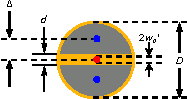
\includegraphics[width = 0.75 \textwidth]{%
    Chapters/InterferometricMethods/figs/phase_plate_beam_separation.pdf}
  \caption[Transverse phase-plate dimensions]{%
    Transverse phase-plate dimensions.
    The unscattered beam is shown in red, while
    the scattered beams are shown in blue.}
  \label{fig:InterferometricMethods:phase_plate_beam_separation}
\end{figure}


\subsection{High-$k$ cutoff of phase plate}
Let the phase plate have a diameter $D$, as is shown in
Fig.~\ref{fig:InterferometricMethods:phase_plate_beam_separation}.
Detection of the scattered radiation
requires that (most of) the scattered beam reflect
from the face of the phase plate
(e.g.\ $\Delta \leq D / 2$).
Application of the phase-plate beam-separation formula
(\ref{eq:InterferometricMethods:phase_plate_beam_separation})
then shows that there will be finite PCI response for $|k| \leq k_D$ where
\begin{equation}
  k_D \equiv \frac{k_0 D}{2 f}.
  \label{eq:InterferometricMethods:pci_kmax_engineering}
\end{equation}


\subsection{Effect of phase plate on $m$\ts{th} scattered beam}
The effect of the PCI phase plate on the $m$\ts{th} scattered beam
is given by the complex-valued function $\mathcal{E}(\vect{r}_m, k)$,
which is derived and thoroughly discussed in
Appendix~\ref{app:PCIResponseIdentities}.
The relevant results are briefly summarized here for completeness.
Eq.~(\ref{eq:PCIResponseIdentities:transformation_Hermitian_decomposed})
shows that PCI's image-plane $\mathcal{E}(\vect{r}_m, k)$
readily reduces to
\begin{equation}
  \begin{aligned}
    \mathcal{E}(\vect{r}_{m,\image}, k_{\image})
    &=
    e^{-[x_{m,\image} / w(z_{m,\image})]^2}
    e^{i m k_{\image} x_{\image}}
    \\
    &\quad\times
    \left[%
      F(\vect{r}_{m,\image}, k_{\image})
      +
      G(\vect{r}_{m,\image}, k_{\image})
    \right],
  \end{aligned}
  \label{eq:InterferometricMethods:PCI_transformation_Hermitian_decomposed}
\end{equation}
where the phase-plate face acts on the $m$\ts{th} scattered beam via $F$, and
the phase-plate groove acts on the $m$\ts{th} scattered beam via $G$.
$F$ and $G$ are themselves defined in
(\ref{eq:PCIResponseIdentities:transformation_face}) and
(\ref{eq:PCIResponseIdentities:transformation_groove}).
Of particular note, $F$ is Hermitian with respect to $m$
\begin{equation}
  F(\vect{r}_{-m,\image}, k_{\image})
  =
  F^*(\vect{r}_{m,\image}, k_{\image}),
  \label{eq:InterferometricMethods:mth_beam_interaction_with_face_hermitian}
\end{equation}
while $G$ is anti-Hermitian with respect to $m$
\begin{equation}
  G(\vect{r}_{-m,\image}, k_{\image})
  =
  -G^*(\vect{r}_{m,\image}, k_{\image}).
  \label{eq:InterferometricMethods:mth_beam_interaction_with_groove_antihermitian}
\end{equation}
These symmetries imply
that $F(\vect{r}_{0,\image}, k_{\image})$ is purely \emph{real} and
that $G(\vect{r}_{0,\image}, k_{\image})$ is purely \emph{imaginary}.


\subsection{The imaged field and its intensity}
\label{sec:InterferometricMethods:pci:imaged_field_and_intensity}
Introducing the notational shorthand
$F_m \equiv F(\vect{r}_{m,\image}, k_{\image})$ and
$G_m \equiv G(\vect{r}_{m,\image}, k_{\image})$,
the weak-coupling ($\tilde{\phi}_0 \ll 1$), image-plane electric field from
(\ref{eq:InterferometricMethods:imaged_total_field_weak_coupling_Fourier_filtered})
readily reduces to
\begin{equation}
  \begin{aligned}
  E(\vect{r}_{\image}, t)
  \approx
  E_G(\vect{r}_{\image}, t)
  e^{i \bar{\phi}}
  \biggl\{%
    F_{0} + G_{0}
    &+
    i \frac{\tilde{\phi}_0}{2}
    \biggl[
      (F_{1} + G_{1}) e^{i \nu}
      \\
      &+
      (F_{-1} + G_{-1}) e^{-i \nu}
    \biggr]
  \biggr\},
  \end{aligned}
\end{equation}
where the approximation $w(z_m) \approx w(z)$ has been used,
$\nu$ is defined in (\ref{eq:InterferometricMethods:image_plane_nu}), and
$E_G(\vect{r}_{\image}, t)$ would be the image-plane electric field
of the unscattered beam in the \emph{absence} of the phase plate.
Now, recall that $F$ is Hermitian such that
$F_{-1} = F^{*}_{1}$ and $F_{0} = \real(F_{0})$ and
that $G$ is anti-Hermitian such that
$G_{-1} = -G^{*}_{1}$ and $G_{0} = {i \cdot \imag(G_{0})}$;
using these substitutions, the field further reduces to
\begin{equation}
  \begin{aligned}
    E(\vect{r}_{\image}, t)
    =
    E_G(\vect{r}_{\image}, t)
    e^{i \bar{\phi}}
    \biggl\{%
      &\real(F_0) - \tilde{\phi}_0 \imag(G_1 e^{i \nu})
      \\
      &+
      i \left[ \imag(G_0) + \tilde{\phi}_0 \real(F_1 e^{i \nu}) \right]
    \biggr\},
  \end{aligned}
\end{equation}
and the corresponding intensity, to first order in $\tilde{\phi}_0$, is
\begin{equation}
  \begin{aligned}
    I_{\text{pci}}(\vect{r}_{\image}, t)
    &=
    I_G(\vect{r}_{\image})
    \biggl\{%
      |F_0|^2 + |G_0|^2
      \\
      &
      +
      2 \tilde{\phi}_0
      \bigl[%
        \imag(G_0) \real(F_1 e^{i \nu})
        -
        \real(F_0) \imag(G_1 e^{i \nu})
      \bigr]
    \biggr\},
  \end{aligned}
\end{equation}
where $I_G(\vect{r}_{\image})$
would be the intensity profile (averaged over an optical cycle)
of the unscattered beam in the \emph{absence} of the phase plate.
Using the fact that $e^{i \nu} = \cos\nu + {i \sin\nu}$,
$F_1 = \real(F_1) + {i \cdot \imag(F_1)}$, and
$G_1 = \real(G_1) + {i \cdot \imag(G_1)}$,
the image-plane intensity further reduces to
\begin{equation}
  \begin{aligned}
    I_{\text{pci}}(\vect{r}_{\image}, t)
    &=
    I_G(\vect{r}_{\image})
    \biggl\{%
      |F_0|^2 + |G_0|^2
      \\
      &+
      2 \tilde{\phi}_0
      \left[ \imag(G_0)\real(F_1) - \real(F_0)\imag(G_1) \right] \cos\nu
      \\
      &-
      2 \tilde{\phi}_0
      \left[ \imag(G_0)\imag(F_1) + \real(F_0)\real(G_1) \right] \sin\nu
    \biggr\}.
  \end{aligned}
  \label{eq:InterferometricMethods:PCI_image_plane_intensity_linear_combination_of_sine_and_cosine}
\end{equation}

Note that the linear combination
$C_I \cos \nu - C_Q \sin \nu$ for real $C_I$, $C_Q$, and $\nu$
can be rewritten as
\begin{align}
  C_I \cos \nu - C_Q \sin \nu
  &=
  C \cos(\nu + \theta),
  \label{eq:InterferometricMethods:linear_combination_of_sine_and_cosine}
\end{align}
where
$C = (C_I^2 + C_Q^2)^{1/2}$,
$\theta = \atantwo(C_Q, C_I)$,
and $\atantwo(C_Q, C_I)$ is the arctangent function of two arguments, which
uses the signs of $C_Q$ and $C_I$ to correctly determine the quadrant
corresponding to a tangent of $C_Q / C_I$.
Note that the notation is mnemonic:
$C_I$ is the amplitude of the ``in-phase'' ($I$) component
(i.e.\ proportional to the image of the assumed
cosine phase fluctuation $\tilde{\phi}(x, t)$ from
(\ref{eq:InterferometricMethods:cosine_phase_fluctuation})), and
$C_Q$ is the amplitude of the corresponding ``quadrature'' ($Q$) component.
Taking inspiration from
(\ref{eq:InterferometricMethods:linear_combination_of_sine_and_cosine}),
the image-plane PCI intensity from
(\ref{eq:InterferometricMethods:PCI_image_plane_intensity_linear_combination_of_sine_and_cosine})
can be rewritten as
\begin{equation}
  \begin{aligned}
    I_{\text{pci}}(\vect{r}_{\image}, t)
    &\approx
    I_G(\vect{r}_{\image})
    \left( |F_0|^2 + |G_0|^2 \right)
    \\
    &\quad\times
    \left\{%
      1
      +
      T_{\text{pp}}(k_{\image}, x_{\image})
      \cdot
      \tilde{\phi}_0
      \cos\left[ \nu + \theta_{\text{pp}}(k_{\image}, x_{\image}) \right]
    \right\},
  \end{aligned}
\end{equation}
where
\begin{align}
  T_{\text{pp}}(k_{\image}, x_{\image})
  &\equiv
  \frac{2 C(k_{\image}, x_{\image})}{|F_0|^2 + |G_0|^2},
  \\
  \theta_{\text{pp}}(k_{\image}, x_{\image})
  &\equiv
  \atantwo(C_Q, C_I),
\end{align}
and
\begin{align}
  C(k_{\image}, x_{\image})
  &\equiv
  (C_I^2 + C_Q^2)^{1/2},
  \\
  C_I(k_{\image}, x_{\image})
  &\equiv
  \imag(G_0)\real(F_1) - \real(F_0)\imag(G_1),
  \label{eq:InterferometricMethods:PCI_response_CI}
  \\
  C_Q(k_{\image}, x_{\image})
  &\equiv
  \imag(G_0)\imag(F_1) + \real(F_0)\real(G_1).
  \label{eq:InterferometricMethods:PCI_response_CQ}
\end{align}

Thus, the action of the phase plate results in both
an amplitude response $T_{\text{pp}}(k_{\image}, x_{\image})$ and
a phase response $\theta_{\text{pp}}(k_{\image}, x_{\image})$
in PCI's image-plane intensity.
The on-axis responses $T_{\text{pp}}(k_{\image}, x_{\image} = 0)$ and
$\theta_{\text{pp}}(k_{\image}, x_{\image} = 0) = 0$
are consistent with previous derivations at $x_{\image} = 0$,
such as \cite[Eq.~2.141]{coda_phd} and \cite[Eq.~20]{rost_low_k_pci}.
The present work, however, explicitly accounts for
the spatial variation in the amplitude and phase responses
across the face of the detector.
Note that $I_{\text{pci}}$ will be a nonlinear function
of the scattering phase fluctuation $\tilde{\phi}(x, t)$
if there are substantial spatial variations in either
$T_{\text{pp}}$ or $\theta_{\text{pp}}$.
The amplitude and phase responses
can be easily evaluated numerically, and
the results for typical system parameters are shown in
Fig.~\ref{fig:InterferometricMethods:phase_plate_amplitude_and_phase_response}.
As is colloquially understood, the amplitude response
drops precipitously across the full beam profile for $k \lesssim k_g$.
(Additionally, the spatial variation in the amplitude response is minimal;
that is,
$T_{\text{pp}}(k_{\image}, x_{\image})
\approx
T_{\text{pp}}(k_{\image}, x_{\image} = 0)$,
particularly for $|k| \gtrsim 2 k_g$).
However, perhaps less well known, is the fact that
the phase response varies substantially in space for $|k| \lesssim k_g$.
Thus, PCI's operation for $|k| \lesssim k_g$ is \emph{nonlinear} and
cannot be described in terms of a transfer function;
this can e.g.\ prevent PCI from measuring wavenumbers
of low-$k$ coherent MHD modes, as is discussed in
Section~\ref{sec:InterferometricMethods:selection:pci_low_k_upshift}.
\graffito{\textcolor{red}{Is this just when $k_g = 2 / w_0$? Or arbitrary $k_g$?}}
Fortunately, for $|k| \gtrsim 2 k_g$, spatial variations
in $\theta_{\text{pp}}$ (and $T_{\text{pp}}$) are negligible, and,
as a result, PCI's operation is essentially linear and
can be described in terms of a transfer function.

\begin{figure}
  \centering
  \includegraphics[width = \textwidth]{%
    Chapters/InterferometricMethods/figs/phase_plate_amplitude_and_phase_response.pdf}
    \caption[Amplitude and phase responses of PCI image-plane intensity
      across detector face
    ]{%
    Amplitude response $T_{\text{pp}}(k, x_{\image})$ and
    phase response $\theta_{\text{pp}}(k, x_{\image})$
    of PCI image-plane intensity across detector face
    for a single sinusoidal mode of wavenumber $k$.
    Spatial coordinates are normalized
    to the image-plane 1/e $E$ radius $M w_0$ with $M = 0.5$, while
    object-plane wavenumbers $k$ are normalized
    to the 1/e $E$ radius of the in-vessel probe beam, $w_0$.
    The horizontal, dashed lines indicate
    the low-$k$ cutoff of the PCI phase-plate groove, $k_g$;
    here, $k_g = 2 / w_0$,
    which is the minimum value allowed by diffraction,
    as discussed in
    (\ref{eq:InterferometricMethods:pci_kmin_physics}).
    The phase-plate high-$k$ cutoff, $k_D$,
    is taken to be much larger than $10 / w_0$.
    The reflectivity of the PCI phase groove is $\eta = 0.17$,
    which is characteristic of the ZnSe typically
    employed in $\SI{10.6}{\micro\meter}$ optics.
    Note that the low-$k$ phase response exhibits dramatic spatial variation,
    which results in nonlinear PCI operation for $|k| \lesssim k_g$.
  }
\label{fig:InterferometricMethods:phase_plate_amplitude_and_phase_response}
\end{figure}


\subsection{The PCI ``transfer function''}
As was the case for external reference-beam interferometry,
it is useful to characterize PCI's performance
relative to the saturation limits of a given detector.
Assume that PCI's imaged field impinges on a detector array,
as shown in Fig.~\ref{fig:InterferometricMethods:detector_array}.
Let the $j$\ts{th} detector element $D_j$ be centered on $x_{\image,j}$
and $y_{\image} = 0$;
the total power $P_{j, \, \text{pci}}$ incident on this element is then
\begin{align}
  P_{j, \, \text{pci}}(t)
  &=
  \int_{D_j} I_{\text{pci}}(\vect{r}_{\image}, t) dA
  \notag
  \\
  &\begin{aligned}
    &\approx
    I_G(\vect{r}_{\image,j})
    \left( |F_0|^2 + |G_0|^2 \right)
    s_y
    \\
    &\quad\times
    \int_{x_{\image,j} - s_x / 2}^{x_{\image,j} + s_x / 2}
    \left\{
      1
      +
      T_{\text{pp}}
      \cdot
      \tilde{\phi}_0
      \cos\left[ \nu + \theta_{\text{pp}} \right]
    \right\} dx_{\image}
  \end{aligned}
  \notag
  \\
  &\begin{aligned}
    &\approx
    I_G(\vect{r}_{\image,j})
    \left( |F_0|^2 + |G_0|^2 \right)
    A
    \\
    &\quad\times
    \left\{
      1
      +
      T_{\text{fsv}}
      T_{\text{pp},j}
      \cdot
      \tilde{\phi}_0
      \cos\left[ \nu_j + \theta_{\text{pp},j} \right]
    \right\},
  \end{aligned}
  \label{eq:InterferometricMethods:PCI_total_power_per_element}
\end{align}
where the weakly varying intensity profile $I_G(\vect{r}_{\image})$
has been approximated as a constant
over the face of the detector element,
the finite sampling-volume integral in
(\ref{eq:InterferometricMethods:finite_sampling_volume_integral})
has been referenced, and
the following abbreviations have been used:
$T_{\text{pp}} = T_{\text{pp}}(k_{\image}, x_{\image})$,
$\theta_{\text{pp}} = \theta_{\text{pp}}(k_{\image}, x_{\image})$,
$T_{\text{fsv}} = T_{\text{fsv}}(k_{\image})$,
$T_{\text{pp},j} = T_{\text{pp}}(k_{\image}, x_{\image,j})$, and
$\theta_{\text{pp},j} = \theta_{\text{pp}}(k_{\image}, x_{\image,j})$.
Because $\tilde{\phi}_0 \ll 1$,
the optical power incident on the $j$\ts{th} detector element
(\ref{eq:InterferometricMethods:PCI_total_power_per_element})
satisfies
\begin{align}
  P_{j, \, \text{pci}}(t)
  &\lesssim
  I_G(0)
  \left( |F_0|^2 + |G_0|^2 \right)
  A,
  \notag
\end{align}
where $I_G(0)$ is the peak intensity
of the unscattered Gaussian probe beam
in the \emph{absence} of the phase plate.
To obtain optimal performance, select $I_G(0)$ such that
\begin{equation}
  P_{\text{sat}}
  =
  I_G(0)
  \left( |F_0|^2 + |G_0|^2 \right)
  A,
  \notag
\end{equation}
where $P_{\text{sat}}$ is the saturation power of a single detector element.
Further, define the fluctuating power in the PCI signal to be
\begin{equation}
  \begin{aligned}
    \tilde{P}_{j, \, \text{pci}}(t)
    &\equiv
    I_G(\vect{r}_{\image,j})
    \left( |F_0|^2 + |G_0|^2 \right)
    A
    \\
    &\quad\times
    \left\{
      T_{\text{fsv}}
      T_{\text{pp},j}
      \cdot
      \tilde{\phi}_0
      \cos\left[ \nu_j + \theta_{\text{pp},j} \right]
    \right\}
  \end{aligned}
  \label{eq:InterferometricMethods:PCI_fluctuating_power_per_element}
\end{equation}
such that
\begin{equation}
  \frac{\tilde{P}_{j, \, \text{pci}}(t)}{P_{\text{sat}}}
  =
  \frac{I_G(\vect{r}_{\image,j})}{I_G(0)}
  \cdot
  T_{\text{pci}}(k_{\image}, x_{\image, j})
  \cdot
  \tilde{\phi}_0
  \cos\left[ \nu_j + \theta_{\text{pp}}(k_{\image}, x_{\image,j}) \right],
  \label{eq:InterferometricMethods:PCI_ratio_fluctuating_to_equilibrium_power}
\end{equation}
where
\begin{align}
  T_{\text{pci}}(k_{\image}, x_{\image})
  =
  T_{\text{fsv}}(k_{\image})
  \cdot
  T_{\text{pp}}(k_{\image}, x_{\image})
  \label{eq:InterferometricMethods:PCI_wavenumber_transfer_function}
\end{align}
is the PCI's wavenumber ``transfer function''.
Of course, as is discussed in
Section~\ref{sec:InterferometricMethods:pci:imaged_field_and_intensity},
$T_{\text{pci}}$ is only a true transfer function when $|k| \gtrsim 2 k_g$,
for which spatial variations in
$T_{\text{pp}}$ and $\theta_{\text{pp}}$ are negligible and
PCI operates linearly.

As is the case with the homodyne interferometer,
the PCI technique does \emph{not} make an absolute measurement
of the phase-fluctuation amplitude $\tilde{\phi}_0$.
To see this, note that the phase-plate transfer function
$T_{\text{pp}}(k_{\image}, x_{\image})$
depends very sensitively on the system alignment,
with slight excursions of the unscattered beam
from the partially reflective phase-plate groove
onto the fully reflective phase-plate face
resulting in macroscopic changes to the power reaching the detector.
Further, power fluctuations at the beam source
can alter $I_G(\vect{r}_{\image, j})$.
Thus, there are three potentially dynamic quantities:
$\{\tilde{\phi}_0, I_G(\vect{r}_{\image, j}), T_{\text{pp}}\}$,
but there are only two potentially measurable quantities:
the equilibrium and fluctuating powers.
PCI systems on large, vibration-prone fusion devices
typically employ feedback stabilization
(see e.g.~\cite[Ch.~3.5]{coda_phd})
in order to dynamically maintain
the unscattered beam's alignment
on the phase-plate groove,
minimizing vibrational contamination of the PCI signal.
It is then possible, after measuring a calibration constant,
to \emph{estimate} the phase-fluctuation amplitude $\tilde{\phi}_0$ with PCI.


\section{Selecting an interferometric technique}
\label{sec:InterferometricMethods:selection}
Sections~\ref{sec:InterferometricMethods:interferometry}
and~\ref{sec:InterferometricMethods:pci}
detail external reference-beam interferometry and
phase contrast imaging (PCI), respectively.
The intent of this section is to synthesize these results and
to discuss the strengths and limitations
of these interferometric techniques
so that a suitable method can be selected for a given application.


\subsection{A note on notation}
The transfer functions derived in the preceding sections
are all written in terms of image-plane wavenumbers $k_{\image}$ and
image-plane coordinates $x_{\image}$.
However, one is often interested in the object-plane wavenumbers $k$,
as they are directly tied to the underlying physics.
In contrast, image-plane coordinates $x_{\image}$
emphasize the importance of the detector dimensions
on the measured interference signal.
For these reasons, the below discussions
use transfer functions with the ``hybrid'' parametrization of
object-plane wavenumbers $k$ and image-plane coordinates $x_{\image}$.
If the reader favors a different parametrization, however,
the transformations between the image-plane and object-plane quantities
are very simple:
\begin{align}
  k_{\image} &= \frac{k}{M},
  \\
  x_{\image} &= M x_{\object},
\end{align}
where $M$ is the imaging system's magnification.


\subsection{Amplitude of fluctuating signal}
The amplitude of the fluctuating signal at the detector
is one of the two aspects
that determines an interferometric system's
signal-to-noise ratio ($\snr$;
the other aspect is the detector noise).
The interferometric-method transfer functions
were defined in the previous sections
by normalizing the power in the fluctuating signal
to the saturation power of a given detector.
Thus, assuming each interferometric method
is implemented with detectors constrained by the same saturation power,
a true ``apples-to-apples'' comparison
of signal amplitudes can be made
by examining the amplitudes of the corresponding transfer functions.
Just such a comparison is shown in
Fig.~\ref{fig:InterferometricMethods:interferometric_method_transfer_functions}.
To facilitate the comparison,
the magnification $|M|$ and detector-element size $s_x$
are taken to be the same for each system.

\begin{figure}
  \centering
  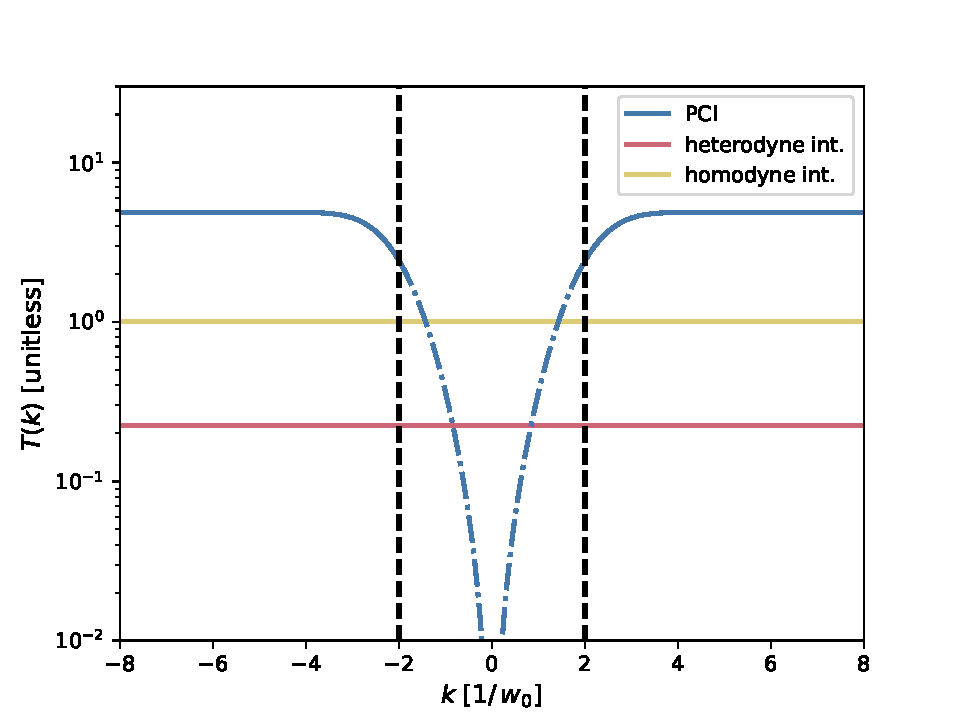
\includegraphics[width = \textwidth]{%
    Chapters/InterferometricMethods/figs/interferometric_method_comparison.pdf}
  \caption[Comparison of interferometric method transfer functions]{%
    A comparison of the transfer-function amplitudes for
    PCI (\ref{eq:InterferometricMethods:PCI_wavenumber_transfer_function}),
    heterodyne interferometry
    (\ref{eq:InterferometricMethods:heterodyne_interferometer_wavenumber_transfer_function}),
    and homodyne interferometry
    (\ref{eq:InterferometricMethods:homodyne_interferometer_wavenumber_transfer_function},
    in the optimal configuration with $\phi_R - \bar{\phi} = \pi / 2$).
    Object-plane wavenumbers $k$ are normalized
    to the 1/e $E$ radius of the in-vessel probe beam, $w_0$.
    Further, to facilitate the comparison,
    the magnification $|M|$ and detector-element size $s_x$
    are taken to be the same for each system
    (specifically, $|M| = 0.5$ and $s_x \approx 0.105 w_0$,
    which are representative ``typical'' values;
    note that these values of $|M|$ and $s_x$
    yield a finite sampling-volume cutoff $k_{\text{fsv}} = 30 / w_0$).
    The vertical, dashed lines indicate
    the low-$k$ cutoff of the PCI phase-plate groove, $k_g$;
    here, $k_g = 2 / w_0$,
    which is the minimum value allowed by diffraction,
    as discussed in
    (\ref{eq:InterferometricMethods:pci_kmin_physics}).
    The phase-plate's high-$k$ cutoff, $k_D$, was assumed to satisfy
    $k_D \gg k_{\text{fsv}}$ such that
    $k_D$ minimally affects the PCI transfer function.
    The reflectivity of the PCI phase groove is $\eta = 0.17$,
    which is characteristic of the ZnSe typically
    employed in $\SI{10.6}{\micro\meter}$ optics.
    As discussed in
    Section~\ref{sec:InterferometricMethods:pci:imaged_field_and_intensity},
    $T_{\text{pci}}$ is only a true transfer function
    for $|k| \gtrsim 2 k_g$;
    for smaller wavenumbers, the PCI phase response
    varies significantly across the beam profile,
    resulting in nonlinear operation.
    Regardless, the PCI ``transfer function'' is plotted
    across the full $k$-range here and
    corresponds to the beam center ($x = 0$).
  }
\label{fig:InterferometricMethods:interferometric_method_transfer_functions}
\end{figure}

Clearly, for a given fluctuation and detector,
PCI produces a fluctuating signal with the largest amplitude.
Relative to the optimally operating homodyne interferometer
($\phi_R - \bar{\phi} = \pi / 2$),
the PCI's larger amplitude is wholly attributable
to the partial reflectivity ($\eta < 1$) of the phase-plate groove:
the decreased power in the unscattered beam
increases the ratio of fluctuating power to equilibrium power
at the PCI detector.
PCI's sensitivity comes with several costs, however.
First, PCI can only measure phase fluctuations,
whereas external reference-beam interferometers
can measure both equilibrium and fluctuating phase.
This makes intuitive sense:
the equilibrium phase uniformly affects
both the scattered and unscattered beams,
the PCI phase delays the unscattered beam
to generate an ``internal'' reference beam, and
the equilibrium phase information cancels in the resulting interference.
Second, PCI depends very sensitively on the system alignment, and
feedback stabilization is often needed
in order to dynamically maintain
the unscattered beam's alignment on the phase-plate groove
(see e.g.~\cite[Ch.~3.5]{coda_phd}).
While this is an added technical complication,
it should be noted that such feedback stabilization
is expected to become more commonplace
for laser diagnostics on large fusion devices,
such as ITER's heterodyne interferometer
\cite{vanzeeland_TIP_rsi13}.
Finally, as was previously discussed,
PCI does not measure the absolute scale of phase fluctuations, but
calibrations can allow estimates of the absolute scale.

The merits and limitations of homodyne and heterodyne interferometry
were discussed at length in
Sec.~{\ref{sec:InterferometricMethods:interferometry}}, but
they are briefly reviewed here for ease of reference.
The homodyne interferometer's transfer function depends on
the difference between the reference-arm phase and
the equilibrium phase, $\phi_R - \bar{\phi}$,
with peak sensitivity when
$\phi_R - \bar{\phi} = \pi / 2$.
However, due to evolution of the equilibrium phase and vibrations,
it is typically difficult to keep $\phi_R - \bar{\phi}$ fixed at $\pi / 2$.
On small fusion devices,
actively controlled mirrors have been used in an attempt
to account for the evolution of the equilibrium phase and
to cancel vibrational path-length changes,
minimizing excursions from $\phi_R - \bar{\phi} \approx \pi / 2$
\cite{nazikian_rsi87}, but
such an approach has not found application on larger
(and presumably more vibration-prone) fusion experiments.
In contrast, the heterodyne interferometer's transfer function
is independent of $\phi_R - \bar{\phi}$.
Further, in contrast to PCI and homodyne interferometry,
the heterodyne interferometer measures
the absolute scale of phase fluctuations,
independent of any calibration constants.
This robust sensitivity and ability to measure absolute phase fluctuations
comes at a cost, however:
a heterodyne interferometer is four times \emph{less} sensitive
than a homodyne interferometer operated in its optimal configuration
($\phi_R - \bar{\phi} = \pi / 2$), which results from
the need to capture the full sinusoidal waveform
of the heterodyne signal at the detector and
the subsequent need to demodulate the heterodyne signal.


\subsection{Spatial bandwidth}
The spatial bandwidth of both homodyne and heterodyne interferometry
is dictated by the system magnification $M$ and
the detector element's length $s_x$;
these parameters give the finite sampling-volume cutoff,
$k_{\text{fsv}} = 2 \pi M / s_x$.
Finite sampling-volume effects also influence PCI's spatial bandwidth.
While $k_{\text{fsv}}$ was specified to be the same
for all of the interferometric systems displayed in
Fig.~\ref{fig:InterferometricMethods:interferometric_method_transfer_functions},
one could easily imagine altering
a given system's magnification $M$ or detector-element size $s_x$
in order to expand or contract the system's spatial bandwidth.

In addition to finite sampling-volume effects,
PCI's spatial bandwidth is also influenced by
the phase plate's low-$k$ and high-$k$ cutoffs,
$k_g$ and $k_D$, respectively.
The effects of $k_g$, $k_D$, and $k_{\text{fsv}}$
are characterized in
Fig.~\ref{fig:InterferometricMethods:pci_cutoffs}.
The most significant effect of the phase plate
on the spatial bandwidth of the PCI
is to introduce a ``hole'' in the low-$k$ response of the system;
external reference-beam interferometers, in contrast,
do not suffer from such a low-$k$ cutoff.
As discussed in
Sec.~\ref{sec:InterferometricMethods:pci:imaged_field_and_intensity},
the PCI also operates nonlinearly in this low-$k$ ``hole'';
one consequence of this nonlinear operation is discussed in
Sec.~\ref{sec:InterferometricMethods:selection:pci_low_k_upshift}.

\begin{figure}
  \centering
  \includegraphics[width = \textwidth]{%
    Chapters/InterferometricMethods/figs/pci_cutoffs.pdf}
  \caption[Effects of phase-plate and finite sampling-volume cutoffs
      on the PCI transfer function]{%
    Effects of the low-$k$ ($k_g$) and high-$k$ ($k_D$) phase-plate cutoffs
    on the phase-plate transfer function, $T_{\text{pp}}(k)$;
    inclusion of finite sampling-volume effects
    then yields the full PCI transfer function, $T_{\text{pci}}(k)$.
    Object-plane wavenumbers $k$ are normalized
    to the 1/e $E$ radius of the in-vessel probe beam, $w_0$.
    The vertical, dashed lines indicate
    the low-$k$ cutoff of the PCI phase-plate groove, $k_g$;
    here, $k_g = 2 / w_0$,
    which is the minimum value allowed by diffraction,
    as discussed in
    (\ref{eq:InterferometricMethods:pci_kmin_physics}).
    The vertical, dashed-dotted lines indicate
    the phase-plate's high-$k$ cutoff,
    chosen here to be $k_D = 20 / w_0$.
    The finite sampling-volume cutoff $k_{\text{fsv}} = 30 / w_0$
    results from representative ``typical'' values of
    system magnification $|M| = 0.5$ and
    detector-element size $s_x \approx 0.105 w_0$.
    Note that here $k_D < k_{\text{fsv}}$, in contrast to
    Fig.~\ref{fig:InterferometricMethods:interferometric_method_transfer_functions}.
    The reflectivity of the PCI phase groove is $\eta = 0.17$,
    which is characteristic of the ZnSe typically
    employed in $\SI{10.6}{\micro\meter}$ optics.
    As discussed in
    Section~\ref{sec:InterferometricMethods:pci:imaged_field_and_intensity},
    $T_{\text{pp}}$ and $T_{\text{pci}}$ are only true transfer functions
    for $|k| \gtrsim 2 k_g$;
    for smaller wavenumbers, the PCI phase response
    varies significantly across the beam profile,
    resulting in nonlinear operation.
    Regardless, the corresponding ``transfer functions'' are plotted
    across the full $k$-range here and
    correspond to the beam center ($x = 0$).
  }
\label{fig:InterferometricMethods:pci_cutoffs}
\end{figure}

Finally, it should be noted that the above transfer functions
have all been computed assuming that the beams are \emph{not} clipped
by apertures in their corresponding optical trains.
Aperture diffraction minimally affects Gaussian beam propagation if
\begin{equation}
  a_{\text{eff}} \geq \frac{3}{2} w(z),
  \label{eq:InterferometricMethods:aperture_radius_for_minimal_diffraction}
\end{equation}
where $a_{\text{eff}}$ is the effective aperture radius and
$w(z)$ is the beam's 1/e $E$ radius at the location of the aperture
\cite{campbell_josa69, rost_diffraction_pc14}.


\subsection{Nonlinear upshift in low-$k$, PCI-measured wavenumber}
\label{sec:InterferometricMethods:selection:pci_low_k_upshift}
This section discusses a little-known diagnostic artifact of the PCI
that becomes relevant when the fluctuation wavenumber
is smaller than the PCI's low-$k$ cutoff (i.e.\ $|k| \lesssim k_g$).
This effect can be important when trying to measure the wavenumber of
e.g.\ low-$k$ coherent MHD modes, and
it results from PCI's nonlinear operation for $|k| \lesssim k_g$,
which is thoroughly discussed in
Section~\ref{sec:InterferometricMethods:pci:imaged_field_and_intensity}.

It is easiest to see the effects of PCI's nonlinear low-$k$ operation
by defining the normalized fluctuating power
$\tilde{p}_j(t)$
\begin{align}
  \tilde{p}_j(t)
  &=
  \frac{I_G(0)}{I_G(\vect{r}_{\image,j})}
  \cdot
  \frac{1}{\tilde{\phi}_0 |T_{\text{pci}}(k_{\image}, x_{\image, j})|}
  \left[ \frac{\tilde{P}_{j, \, \text{pci}}(t)}{P_{\text{sat}}} \right]
  \notag \\
  &=
  \cos\left[ \nu_j + \theta(k_{\image}, x_{\image, j}) \right].
\end{align}
(This choice of normalization becomes readily apparent after referencing
(\ref{eq:InterferometricMethods:PCI_ratio_fluctuating_to_equilibrium_power})).
The set of measurements $\{\tilde{p}_j(t)\}$
can be e.g.\ Fourier analyzed in the spatial dimension
to provide an estimate of the corresponding
wavenumber autospectral density
$G_{\tilde{p}\tilde{p}}(k_{\text{meas}}, t)$.
\graffito{\textcolor{red}{more details on $G_{xx}(k)$ in Ch.~4}}
When PCI operates linearly,
the measured wavenumber spectrum
has a peak at $k_{\text{meas}} = k$,
with $k$ corresponding to the true, physical wavenumber.
As shown in Fig.~\ref{fig:InterferometricMethods:pci_wavenumber_upshift},
PCI operates linearly for $k \gtrsim k_g$,
as the measured wavenumber spectrum peaks at $k_{\text{meas}} = k$;
however, for $k \lesssim k_g$,
the measured wavenumber spectrum peaks at $k_{\text{meas}} = k_g$,
regardless of the actual fluctuation wavenumber.
The explanation for this effect is relatively simple:
a Gaussian beam can be decomposed into a set of infinite plane waves
traveling in slightly different directions \cite[Ch.~16.7]{siegman_lasers},
and only the components of the scattered beam
with transverse lab-frame wavenumbers $k \geq k_g$
are reflected from the phase-plate face and
produce measurable interference on the PCI detector.
Thus, when $|k| \lesssim k_g$,
not only does the PCI signal's amplitude drop precipitously, but
its spatial content also becomes a nonlinear function
of the corresponding fluctuation wavenumber,
destroying any hopes of wavenumber measurement.

\begin{figure}
  \centering
  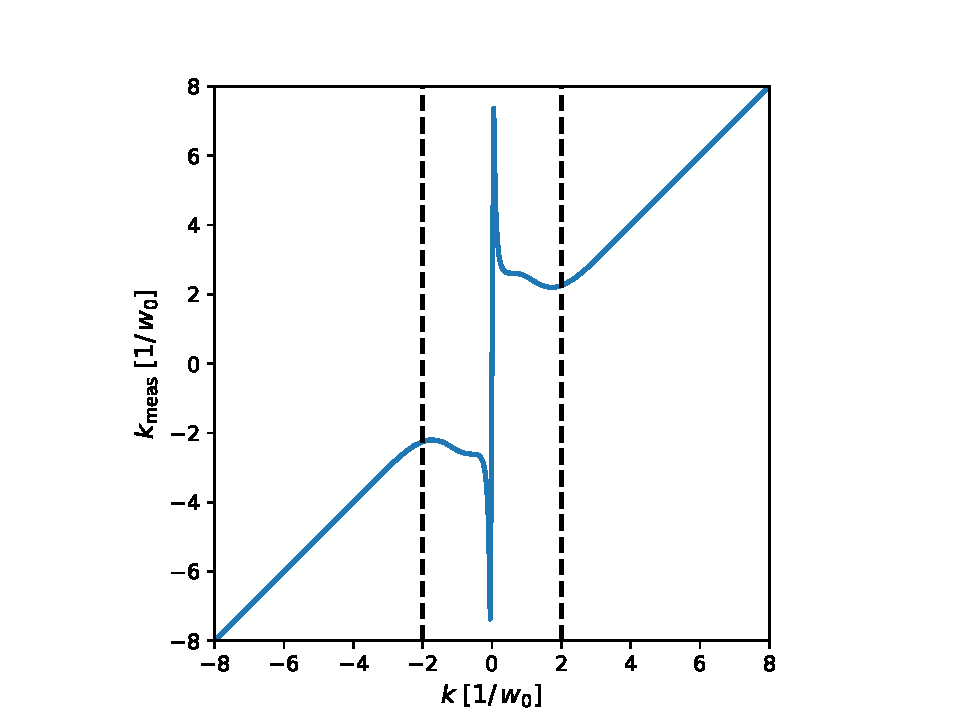
\includegraphics[width = \textwidth]{%
    Chapters/InterferometricMethods/figs/pci_wavenumber_upshift.pdf}
    \caption[Nonlinear upshift in low-$k$, PCI-measured wavenumber]{%
    Estimate of wavenumber autospectral density $G_{\tilde{p}\tilde{p}}(k)$
    that results from Fourier analyzing
    the normalized PCI signal $\tilde{p}$ in space.
    The $y$-axis displays the fluctuation's actual wavenumber $k$, while
    the $x$-axis displays the corresponding ``measured'' wavenumber
    $k_{\text{meas}}$ that results from the Fourier analysis.
    Wavenumbers are all normalized
    to the 1/e $E$ radius of the in-vessel probe beam, $w_0$.
    The horizontal, dashed line indicates
    the low-$k$ cutoff of the PCI phase-plate groove, $k_g$;
    here, $k_g = 2 / w_0$,
    which is the minimum value allowed by diffraction,
    as discussed in
    (\ref{eq:InterferometricMethods:pci_kmin_physics}).
    The system magnification has
    a representative ``typical'' value $|M| = 0.5$.
    Note that PCI operates linearly for $k \gtrsim k_g$,
    as the measured wavenumber spectrum peaks at $k_{\text{meas}} = k$;
    however, for $k \lesssim k_g$,
    the measured wavenumber spectrum peaks at $k_{\text{meas}} = k_g$,
    regardless of the actual fluctuation wavenumber.
  }
\label{fig:InterferometricMethods:pci_wavenumber_upshift}
\end{figure}


\subsection{Temporal bandwidth}
Finally, the required temporal bandwidth should also be considered.
For heterodyne interferometry,
proper reconstruction of the fluctuating baseband signal
at angular frequency $\omega$
from the heterodyne signal
at angular intermediate frequency $\Delta \omega_0$ requires that
$\omega < \Delta \omega_0$.
Further, the detector's angular cutoff frequency $\omega_{\text{det}}$
should be sufficiently large to capture the relevant dynamics such that
\begin{equation}
  \omega_{\text{det}} > \Delta \omega_0 + \omega,
  \qquad
  \text{heterodyne interferometry.}
\end{equation}
In contrast, homodyne interferometry and PCI only require that
\begin{equation}
  \omega_{\text{det}} > \omega,
  \qquad \qquad \quad% \qquad
  \text{homodyne interferometry, PCI.}
\end{equation}
Thus, heterodyne interferometry requires a faster detector
than homodyne interferometry or PCI\@.
For the HgCdTe detectors typically used at $\SI{10.6}{\micro\meter}$,
cooling the active element of the detector
reduces detector noise and increases the detector response
but also reduces $\omega_{\text{det}}$.
Thus, for low-temporal-bandwidth applications,
homodyne interferometry and PCI can use
slower, cooled detectors that will improve
system signal-to-noise ratio ($\snr$)
relative to the faster, warmer detectors
required for heterodyne interferometry.
Deployment of homodyne interferometry or PCI
in high-temporal-bandwidth applications, however,
requires the use of higher bandwidth detectors and/or
more exotic detection techniques, such as
optical heterodyning~\cite[Sec.~3.3.1]{tsujii_phd}.


\bibliographystyle{plainurl}
\bibliography{references}
